\documentclass[conference]{IEEEtran}
\IEEEoverridecommandlockouts
% Overleaf-compatible: upload the whole report/ folder (main.tex, sections/, tables/, figures/, refs.bib).
\usepackage{cite}
\usepackage{amsmath,amssymb,amsfonts}
\usepackage{algorithm}
\usepackage{algpseudocode}
\usepackage{graphicx}
\usepackage{booktabs}
\usepackage{multirow}
\usepackage{xcolor}
\usepackage{tikz}
\usetikzlibrary{arrows.meta,positioning,fit,backgrounds}
\usepackage{url}
\usepackage[hidelinks]{hyperref}
\graphicspath{{figures/}}
\newcommand{\sys}{\textsc{EligiTrace}}

\begin{document}

\title{\sys: Evidence-Traced Clinical-Trial Eligibility Screening with a Fine-Tuned Small Language Model, KV-Cached and Speculative Decoding, and Tiled Online-Softmax Attention}

\author{\IEEEauthorblockN{Muhammad Ruhan Kamran}
\IEEEauthorblockA{\textit{Department of Computer Science} \\
\textit{FAST University (NUCES) Islamabad}\\
Islamabad, Pakistan \\
Roll No. 23i-0062, Section CS-A}}

\maketitle

\begin{abstract}
Pre-screening patients for clinical trials means checking a free-text note against every eligibility criterion
and citing the facts that justify each decision. We present \sys, a locally executable system for
criterion-level eligibility prediction with evidence tracing, built on Qwen2.5-1.5B-Instruct and the TrialGPT
criterion-annotation benchmark. We fine-tune the model with LoRA on a 6\,GB consumer GPU, choosing bf16 with
gradient checkpointing after measuring the alternatives. On held-out test patients, the same model goes from
0.160 to 0.733 accuracy, from 0.155 to 0.528 macro-F1 over the labels present, and from 0.169 to 0.561
evidence micro-F1, with no unparseable outputs. We also implement and benchmark three inference mechanisms by
hand:
\begin{itemize}
\item a KV-cached decoder, $3.6\times$ faster than recomputation at 128 context tokens and up to $20\times$ at
1{,}024;
\item a tiled online-softmax attention kernel that matches a float64 reference to $2.5\times10^{-6}$ in fp32 and uses
46$\times$ less memory than unfused attention at 4{,}096 tokens;
\item a greedy speculative decoder whose draft acceptance reaches 91\% (96\% with a fine-tuned draft), but
which is still slower than plain cached decoding on launch-bound consumer hardware.
\end{itemize}
Where bf16 outputs diverge from the reference, we trace the cause to logit ties within one bf16 rounding
step and confirm exact agreement in fp32. A browser application screens unseen notes, highlights evidence
sentences, explains each decision only from the cited evidence, and exposes the inference mechanisms live.
\end{abstract}

\begin{IEEEkeywords}
clinical-trial matching, LoRA, KV cache, speculative decoding, online softmax, evidence attribution
\end{IEEEkeywords}

\section{Introduction and Problem Statement}\label{sec:intro}
Clinical trials fail to recruit on time far more often than they fail scientifically, and a large part
of the recruitment burden is \emph{pre-screening}: a coordinator reads a free-text patient note against
every inclusion and exclusion criterion of a protocol. The task is criterion-level, evidence-heavy and
asymmetric---an absent fact is not a negative fact. Large proprietary models have shown strong results on
this problem~\cite{jin2024trialgpt,wornow2024zeroshot}, but they cannot be run locally on protected data,
are expensive, and expose no control over inference.

We study the problem as defined by the TrialGPT criterion-annotation benchmark~\cite{jin2024trialgpt}:
given (i) a patient note split into numbered sentences, (ii) a criterion type (inclusion or exclusion) and
(iii) the criterion text, predict the expert eligibility label---one of four type-specific categories,
including \emph{not enough information} and \emph{not applicable}---and the IDs of the patient sentences
that support it. A deployable answer must also be \emph{traceable}: each decision should point at its
evidence and explain itself only from that evidence.

\textbf{Contributions.} We present \sys, a complete, locally executable system built around
Qwen2.5-1.5B-Instruct~\cite{qwen2025qwen25}:
\begin{enumerate}
\item a leakage-safe data pipeline and the prescribed patient-grouped 37/8/8 split with a published
manifest and automated leakage tests;
\item a LoRA~\cite{hu2022lora} adaptation whose precision strategy was \emph{chosen by measurement} on a
6\,GB consumer GPU, with a same-model before/after comparison on identical held-out examples;
\item a hand-written KV-cached greedy decoder, a tiled online-softmax attention kernel and a greedy
speculative decoder, each validated against a reference (exact in fp32, and in bf16 up to logit ties within one rounding
step) and benchmarked under controlled conditions;
\item a browser application that screens unseen notes against typed or fetched criteria, highlights the
exact evidence sentences, aggregates criterion decisions with an explicit rule, exports a provenance-stamped
report, and exposes a live inference laboratory.
\end{enumerate}
Fig.~\ref{fig:arch} summarises the system.

\section{Related Work}\label{sec:related}
\textbf{Patient--trial matching.} Koopman and Zuccon~\cite{koopman2016test} released the patient topics
that underlie the benchmark used here. TrialGPT~\cite{jin2024trialgpt} decomposes matching into
criterion-level prediction with sentence-level evidence and shows that GPT-4 approaches expert accuracy;
its criterion annotations (expert labels and expert evidence) form our mandatory dataset. Wornow et
al.~\cite{wornow2024zeroshot} reach similar conclusions zero-shot. Both rely on proprietary API models:
excellent accuracy, but no local execution, no control over decoding, and cost per criterion. We instead
ask how far a 1.5\,B-parameter open model adapted on 603 examples can go, and we keep the GPT-4 outputs
shipped with the dataset strictly out of inputs, targets and evaluation.

\textbf{Decoder architectures.} The Transformer~\cite{vaswani2017attention} remains the backbone. Modern
small decoders combine rotary position embeddings (RoPE)~\cite{su2024roformer}, which make attention scores
depend on relative position through rotations applied to queries and keys, and grouped-query attention
(GQA)~\cite{ainslie2023gqa}, which shares key/value heads across query heads and shrinks the KV cache.
Qwen2.5~\cite{qwen2025qwen25}, Llama~3~\cite{grattafiori2024llama3} and Gemma~2~\cite{gemmateam2024gemma2}
all follow this recipe; they differ in licence, vocabulary and the availability of a smaller
same-tokenizer sibling, which matters for speculative decoding (Section~\ref{sec:model}).

\textbf{Parameter-efficient adaptation.} LoRA~\cite{hu2022lora} learns a low-rank update $\Delta W=BA$
for frozen weights, cutting trainable parameters by orders of magnitude; QLoRA~\cite{dettmers2023qlora}
additionally stores the frozen base in 4-bit NF4. Mixed precision~\cite{micikevicius2018mixed} and
gradient checkpointing~\cite{chen2016checkpoint} trade numerical range and recomputation for memory.
These papers report memory and quality on data-centre GPUs; their trade-offs do not transfer directly to
a 6\,GB Turing card without tensor cores, which is why we measure them (Table~\ref{tab:membench}).

\textbf{Efficient inference.} Autoregressive decoding is memory-bandwidth bound; caching keys and values
turns each step from $O(n)$ recomputation into a single-token pass~\cite{pope2023scaling}, and
PagedAttention~\cite{kwon2023paged} manages that cache at serving scale. Online softmax~\cite{milakov2018online}
lets the normaliser be computed in one streaming pass; Rabe and Staats~\cite{rabe2021selfattention} showed
attention needs only $O(\sqrt{n})$ or $O(1)$ extra memory with chunking, and
FlashAttention~\cite{dao2022flashattention,dao2024flashattention2} turned the same idea into fused,
IO-aware GPU kernels. Speculative decoding~\cite{leviathan2023speculative,chen2023speculative} drafts several
tokens with a small model and verifies them in one pass of the large model, preserving the target
distribution exactly (and, for greedy decoding, the exact token sequence). Its benefit depends on the
draft/target cost ratio and the acceptance rate---both of which we measure rather than assume.

\textbf{Limitations of prior work for our setting.} API-based matchers cannot be benchmarked at the
mechanism level; kernel papers report speed on hardware we do not have; and speculative-decoding gains are
reported for large size ratios (e.g.\ 70\,B targets) unlike our 1.5\,B/0.5\,B pair. \sys\ connects these
lines on one consumer GPU and reports where each technique helps and where it does not.

\section{Materials and Methods}\label{sec:methods}

\begin{figure*}[t]
\centering
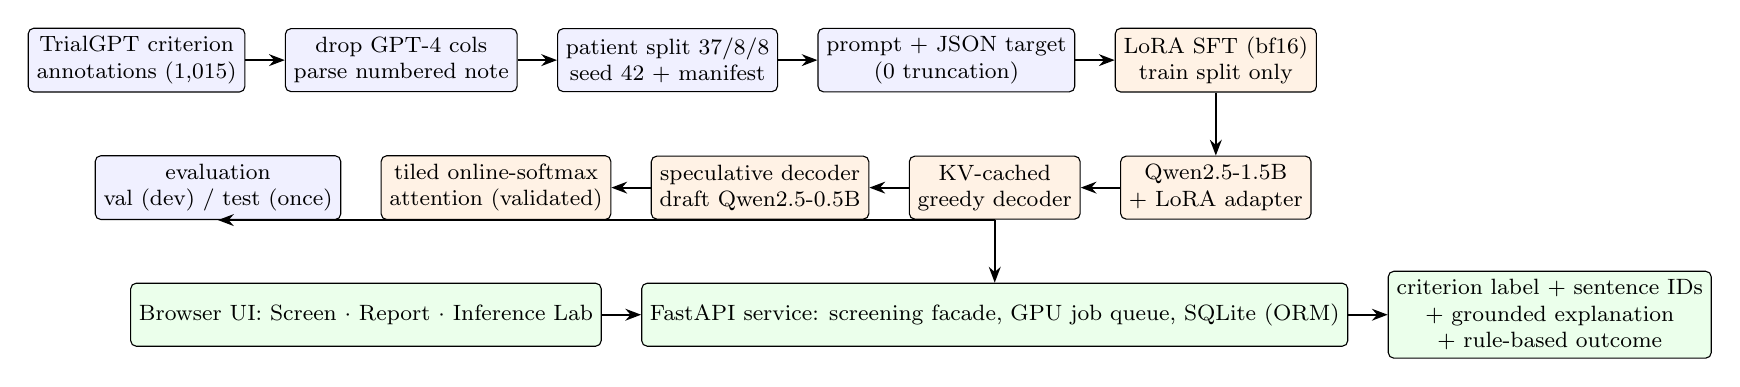
\begin{tikzpicture}[
  node distance=4mm and 5mm, font=\footnotesize,
  box/.style={draw, rounded corners=2pt, align=center, minimum height=8mm, inner sep=3pt, fill=white},
  data/.style={box, fill=blue!6}, model/.style={box, fill=orange!10}, app/.style={box, fill=green!8},
  arr/.style={-{Stealth[length=2mm]}, thick}]
\node[data] (ds) {TrialGPT criterion\\annotations (1{,}015)};
\node[data, right=of ds] (clean) {drop GPT-4 cols\\parse numbered note};
\node[data, right=of clean] (split) {patient split 37/8/8\\seed 42 + manifest};
\node[data, right=of split] (fmt) {prompt + JSON target\\(0 truncation)};
\node[model, right=of fmt] (lora) {LoRA SFT (bf16)\\train split only};
\node[model, below=8mm of lora] (qwen) {Qwen2.5-1.5B\\+ LoRA adapter};
\node[model, left=of qwen] (kv) {KV-cached\\greedy decoder};
\node[model, left=of kv] (spec) {speculative decoder\\draft Qwen2.5-0.5B};
\node[model, left=of spec] (att) {tiled online-softmax\\attention (validated)};
\node[data, left=of att] (eval) {evaluation\\val (dev) / test (once)};
\node[app, below=8mm of kv] (api) {FastAPI service: screening facade, GPU job queue, SQLite (ORM)};
\node[app, left=of api] (ui) {Browser UI: Screen $\cdot$ Report $\cdot$ Inference Lab};
\node[app, right=of api] (out) {criterion label + sentence IDs\\+ grounded explanation\\+ rule-based outcome};
\draw[arr] (ds)--(clean); \draw[arr] (clean)--(split); \draw[arr] (split)--(fmt); \draw[arr] (fmt)--(lora);
\draw[arr] (lora)--(qwen); \draw[arr] (qwen)--(kv); \draw[arr] (kv)--(spec); \draw[arr] (spec.west)--(att.east);
\draw[arr] (kv) |- (eval.south); \draw[arr] (kv)--(api); \draw[arr] (ui)--(api); \draw[arr] (api)--(out);
\end{tikzpicture}
\caption{\sys\ architecture. The offline pipeline (top) prepares leakage-safe data and adapts the model;
the inference core (middle) contains the three hand-written mechanisms; the application (bottom) exposes
screening and live benchmarking in the browser.}
\label{fig:arch}
\end{figure*}

\subsection{Dataset and Leakage Control}\label{sec:data}
We use only \texttt{ncbi/TrialGPT-Criterion-Annotations} (revision \texttt{1cfcafd}). It contains 1{,}015
criterion-level annotations for 53 patients and 103 trials. Notes are already split into numbered sentences
(\texttt{"0. \ldots\textbackslash n1. \ldots"}), so sentence IDs are taken verbatim and evidence is a set of
those IDs. The columns \texttt{gpt4\_explanation}, \texttt{gpt4\_sentences}, \texttt{gpt4\_eligibility},
\texttt{explanation\_correctness} and TrialGPT's own \texttt{training} flag are dropped before any formatting.
A test overwrites all of these columns with a sentinel string and asserts that every one of the 1{,}015
prompts and targets is byte-identical and sentinel-free, proving that model-generated outputs cannot reach the
model. One annotation (ID 883) has an empty criterion text; it is kept, with an explicit marker, so that
counts match the source. Labels are type-specific: inclusion criteria use \{included, not included, not
enough information, not applicable\}; exclusion criteria use \{excluded, not excluded, not enough
information, not applicable\}. The label distribution is highly skewed (e.g.\ only 10 \emph{excluded}).

\subsection{Patient-Grouped Split}\label{sec:split}
Unique patient IDs are sorted lexicographically into a NumPy array, shuffled in place with
\texttt{numpy.random.default\_rng(42)}, and the first 37 / next 8 / last 8 patients form train / validation /
test. Every annotation follows its patient. Table~\ref{tab:split} gives the resulting counts; the manifest
(\texttt{data/splits/split\_manifest.json}) lists patient IDs and a SHA-256 hash of each split's annotation
IDs. Automated tests check sizes, disjointness, full coverage, determinism and that every gold evidence ID
exists in its note. Notably, the test split contains \emph{no} \emph{excluded} example, which affects how
macro-F1 must be read (Section~\ref{sec:metrics}).
\begin{table*}[t]
\centering
\footnotesize
\caption{Patient-grouped split (seed 42) and expert label counts.}
\label{tab:split}
\begin{tabular}{lrrrrrrrrrr}
\toprule
Split & Pat. & Ann. & Inc. & Exc. & incl & not incl & excl & not excl & NEI & N/A \\
\midrule
train & 37 & 603 & 215 & 388 & 88 & 13 & 8 & 292 & 174 & 28 \\
val & 8 & 206 & 66 & 140 & 35 & 3 & 2 & 101 & 53 & 12 \\
test & 8 & 206 & 75 & 131 & 27 & 7 & 0 & 91 & 66 & 15 \\
\bottomrule
\end{tabular}
\end{table*}


\subsection{Model Selection}\label{sec:model}
Table~\ref{tab:candidates} compares five open-weight decoders. Facts are read from each model's
\texttt{config.json}; parameter counts are exact (models instantiated on the \texttt{meta} device, tied
embeddings counted once). We selected \textbf{Qwen2.5-1.5B-Instruct}: Apache-2.0 and ungated; RoPE + GQA with
only 2 KV heads, giving the smallest KV cache of the candidates (28\,KiB/token in 16-bit); a 32\,K context
far above our longest example (623 tokens); 1.54\,B parameters (2.9\,GiB in bf16) that leave room on a 6\,GB
GPU for activations, the KV cache \emph{and} a draft model; and, decisively for Task~5, an official
\textbf{Qwen2.5-0.5B-Instruct} sibling with an identical tokenizer (151{,}665 entries,
identical chat template, identical 151{,}936-wide output layer). Llama-3.2-1B has no smaller same-tokenizer
sibling and a gated community licence; Gemma-2-2B (2.6\,B) and Qwen3-1.7B (1.72\,B, 8 KV
heads $\Rightarrow$ 4$\times$ larger cache) fit less comfortably next to a draft model.
\begin{table*}[t]
\centering
\footnotesize
\caption{Candidate decoders (from config.json; exact parameter counts; 16-bit memory). KV = KiB of cache per token. All use RoPE, RMSNorm/LayerNorm variants and GQA.}
\label{tab:candidates}
\begin{tabular}{lrrcrrrrrl}
\toprule
Model & Params (B) & L & Hq/Hkv & d & Vocab & Ctx & GiB & KV & Licence \\
\midrule
Qwen2.5-1.5B-Instruct & 1.54 & 28 & 12/2 & 128 & 151k & 32k & 2.9 & 28 & Apache-2.0 \\
Qwen2.5-0.5B-Instruct & 0.49 & 24 & 14/2 & 64 & 151k & 32k & 0.9 & 12 & Apache-2.0 \\
Qwen3-1.7B & 1.72 & 28 & 16/8 & 128 & 151k & 40k & 3.2 & 112 & Apache-2.0 \\
Llama-3.2-1B-Instruct & 1.24 & 16 & 32/8 & 64 & 128k & 128k & 2.3 & 32 & Llama 3.2 CL \\
gemma-2-2b-it & 2.61 & 26 & 8/4 & 256 & 256k & 8k & 4.9 & 104 & Gemma ToU \\
\bottomrule
\end{tabular}
\end{table*}


\subsection{Input/Output Format and Tokenisation}\label{sec:format}
One prompt template (Qwen chat format) is shared by fine-tuning, evaluation and the application. The system
message instructs the model to judge one criterion from the numbered note only, to answer \emph{not enough
information} when facts are missing (``missing evidence is never proof''), and to reply with JSON. The user
message contains the numbered note, the criterion type, the criterion text and the four allowed labels for
that type. The target is a compact JSON object, e.g.\
\texttt{\{"label": "included", "evidence": [0, 3]\}}. With Qwen's byte-level BPE tokenizer the longest
training example is 623 tokens (median 311; Fig.~\ref{fig:tokens}); we set \texttt{max\_seq\_len}=1024, so
\textbf{no example is truncated and no evidence sentence is lost}---verified by an audit that would list any
truncated annotation and any gold sentence beyond the cut. A robust parser extracts the first JSON object,
normalises label synonyms, rejects labels not allowed for the criterion type (counted as \emph{invalid}, never
silently mapped), and drops cited IDs that do not exist in the note (reported as unsupported citations).

\begin{figure}[t]
\centering
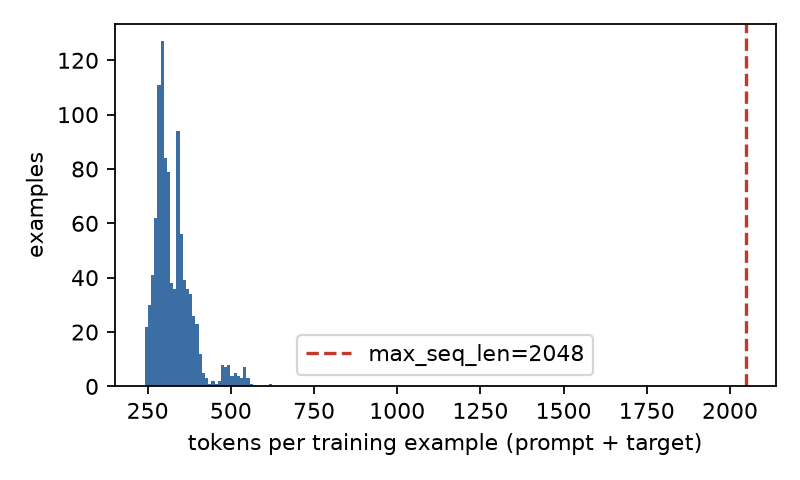
\includegraphics[width=0.92\linewidth]{token_hist.png}
\caption{Tokens per training example (prompt + target) across all 1{,}015 annotations. The dashed line is
the training limit; every example fits, so truncation never removes evidence.}
\label{fig:tokens}
\end{figure}

\subsection{Fine-Tuning}\label{sec:ft}
\textbf{Objective.} Supervised fine-tuning with the causal LM cross-entropy computed only on assistant
(target) tokens; all prompt tokens are masked with $-100$, so the model learns to emit the label and
evidence, not to reproduce notes. The \texttt{<|im\_end|>} token is part of the target, teaching the model
to stop.

\textbf{Precision strategy chosen by measurement.} Our GTX~1660~SUPER (6\,GB, Turing \texttt{sm\_75}, no
tensor cores) behaves unlike the GPUs in the literature. A micro-benchmark gave 3.9\,TFLOP/s for fp32 GEMM,
2.1 for bf16 but only 0.43 for fp16 (cuBLAS fp16 with fp32 accumulation is slow on TU116). We therefore ran
every candidate training configuration for four optimizer steps on the \emph{longest} training example in
a fresh process (Table~\ref{tab:membench}). The Windows driver's ``CUDA sysmem fallback'' initially let fp32
silently spill into system RAM (a 100$\times$ slowdown instead of an error); capping the allocator at the
physical VRAM made out-of-memory explicit. Full fp32 does not fit (6.2\,GiB of weights); accelerate's CPU
offload is incompatible with PEFT gradients; fp16 autocast works but is 3.6$\times$ slower; QLoRA saves
0.9\,GB but quantises the frozen weights. \textbf{bf16 storage of the frozen base + fp32 LoRA weights +
bf16 autocast + gradient checkpointing} is the fastest configuration that keeps the original weights; any
micro-batch above one exceeds memory because the 151{,}936-way output logits dominate activations, so we use
micro-batch 1 with 16 accumulation steps.
\begin{table}[t]
\centering
\footnotesize
\caption{Measured training configurations on NVIDIA GeForce GTX 1660 SUPER (6.0 GB): LoRA r=16, longest training example (623 tokens), 4 optimizer steps, first step excluded from timing.}
\label{tab:membench}
\begin{tabular}{lcrrrrl}
\toprule
Strategy & Ckpt & MB & Weights GiB & Peak GiB & s/step & Status \\
\midrule
fp32 & yes & 1 & -- & -- & -- & OOM \\
fp32-offload & yes & 1 & -- & -- & -- & incompatible \\
fp16-mixed & yes & 1 & 2.94 & 4.22 & 13.80 & ok \\
bf16-mixed & no & 1 & -- & -- & -- & OOM \\
bf16-mixed & yes & 1 & 2.94 & 4.22 & 3.87 & ok \\
bf16-mixed & yes & 4 & -- & -- & -- & OOM \\
bf16-mixed & yes & 8 & -- & -- & -- & OOM \\
qlora-nf4 & yes & 1 & 1.58 & 3.33 & 3.71 & ok \\
qlora-nf4 & yes & 4 & -- & -- & -- & OOM \\
\bottomrule
\end{tabular}
\end{table}


\textbf{Hyper-parameters} (Table~\ref{tab:hparams}): LoRA rank 16, $\alpha$=32, dropout 0.05 on all seven
attention and MLP projections (18.5\,M trainable parameters, 1.2\% of the model), AdamW~\cite{loshchilov2019adamw}
with learning rate $2\times10^{-4}$, cosine schedule with 5\% warm-up, gradient clipping at 1.0, 3 epochs,
seed 42. After each epoch the adapter is saved and the \emph{validation} split is decoded with the exact
evaluation decoder; the epoch with the best validation macro-F1 (ties: evidence micro-F1) is selected.
The test split is never used for selection.
\begin{table}[t]
\centering
\footnotesize
\caption{Fine-tuning configuration.}
\label{tab:hparams}
\begin{tabular}{ll}
\toprule
Setting & Value \\
\midrule
Base model & Qwen/Qwen2.5-1.5B-Instruct \\
Precision & bf16 base, fp32 LoRA, bf16 autocast \\
LoRA r / $\alpha$ / dropout & 16 / 32 / 0.05 \\
Target modules & q,k,v,o,gate,up,down \\
Optimizer & AdamW, wd 0.0 \\
LR / schedule & 0.0002 / cosine, 5\% warm-up \\
Batch & 1 $\times$ 16 accumulation \\
Epochs / clip / seed & 3 / 1.0 / 42 \\
Max length & 1024 (no truncation) \\
Grad. checkpointing & True \\
Selection & best val macro-F1 over epochs \\
\bottomrule
\end{tabular}
\end{table}


\subsection{Grounded Explanations}\label{sec:explain}
The dataset's only free-text explanations are GPT-4 outputs, which we refuse to use as targets (leakage,
and 124 of them are marked partially correct or incorrect). The fine-tuned model therefore emits only label
and evidence, and the explanation is produced afterwards in one of two ways. (i) \emph{Grounded LLM}: the
same network with the LoRA adapter \emph{disabled} (i.e.\ the instruction-tuned base) receives only the
criterion, the decided label and the text of the cited sentences, and writes one or two sentences. A
deterministic grounding check rejects any rationale that mentions a number absent from the cited evidence or
the criterion, or that contradicts the label. (ii) \emph{Template}: a deterministic sentence quoting the cited
evidence verbatim. Rejected LLM rationales fall back to the template, so every explanation shown is grounded
in the cited sentences.

\subsection{KV-Cached Autoregressive Decoding}\label{sec:kv}
We implement greedy decoding directly on model forward passes (Alg.~\ref{alg:kv}). In prefill the full prompt
of length $T$ is processed with \texttt{position\_ids} $=0..T-1$; each layer stores keys (already rotated by
RoPE) and values in a \texttt{DynamicCache} of shape $[B, H_{kv}, T, d]$. Each decode step feeds only the
newest token with absolute position $T+t$ (\texttt{position\_ids} and \texttt{cache\_position}) and an
attention mask extended by one; the cache grows by one entry per layer. Because RoPE is applied before
caching, cached keys retain their absolute positions; a wrong position for the new query silently changes
the output, which our equality tests would detect. A causal mask is needed in prefill but not for a single
query at the last position. The reference path re-runs the whole sequence without cache at every step.
Assertions check the cache length after prefill and after decoding, and a trace records the layer-0 key
shape at every step (Section~\ref{sec:res-kv}). With GQA, the cache stores $H_{kv}=2$ heads instead of
$H_q=12$: $2\cdot L\cdot H_{kv}\cdot d\cdot 2$\,B $=28$\,KiB per token for $L$=28, $d$=128.

\begin{algorithm}[t]
\caption{KV-cached greedy decoding (batch 1)}\label{alg:kv}
\begin{algorithmic}[1]
\State $C\gets$ empty cache; $\ell \gets f(x_{0:T};\ \mathrm{pos}=0..T{-}1, C)$ \Comment{prefill, appends $T$ K/V}
\State $y_1\gets\arg\max \ell_{T-1}$
\For{$t=1$ \textbf{to} $N-1$ \textbf{while} $y_t\notin\mathrm{EOS}$}
  \State $\ell\gets f(y_t;\ \mathrm{pos}=T{+}t{-}1, C)$ \Comment{one token; cache grows by 1}
  \State $y_{t+1}\gets\arg\max \ell$
\EndFor
\State \textbf{assert} $|C| = T + |y| - 1$
\end{algorithmic}
\end{algorithm}

\subsection{Tiled Attention with Online Softmax}\label{sec:attn}
The reference computes $S=QK^\top/\sqrt{d}$ in fp32, masks with $-\infty$ (causal convention: query $i$ at
absolute position $S_k-S_q+i$ may see keys $j\le S_k-S_q+i$, which also covers single-token decode), subtracts the
row maximum before exponentiation, normalises, and multiplies by $V$; fully masked rows return zeros. The
tiled kernel (Alg.~\ref{alg:tiled}) never forms $S$: for each block of $B_q$ queries it streams blocks of $B_k$
keys, keeping a running maximum $m$, normaliser $\ell$ and un-normalised output $A$. When a new block raises
the maximum, previous statistics are rescaled by $\alpha=e^{m-m'}$~\cite{milakov2018online,dao2022flashattention}.
Key blocks entirely above the diagonal are skipped; only diagonal blocks are masked. GQA is handled by
repeating KV heads. All accumulation is in fp32.

\begin{algorithm}[t]
\caption{Tiled attention with online softmax (one query block)}\label{alg:tiled}
\begin{algorithmic}[1]
\State $m\gets-\infty,\ \ell\gets0,\ A\gets0$ \Comment{per query row}
\For{each key block $j$ visible under the causal mask}
  \State $S_j\gets Q_iK_j^\top/\sqrt d$; mask inside the diagonal block
  \State $m'\gets\max(m,\mathrm{rowmax}(S_j))$;\ $P\gets e^{S_j-m'}$;\ $\alpha\gets e^{m-m'}$
  \State $\ell\gets\alpha\ell+\mathrm{rowsum}(P)$;\ $A\gets\alpha A+PV_j$;\ $m\gets m'$
\EndFor
\State $O_i\gets A/\ell$;\quad $\mathrm{LSE}_i\gets m+\log\ell$
\end{algorithmic}
\end{algorithm}

\subsection{Greedy Speculative Decoding}\label{sec:spec}
Draft $D$ (Qwen2.5-0.5B-Instruct, 0.49\,B) and target $M$ (fine-tuned 1.5\,B) keep separate KV caches. With
$s$ the current sequence of length $L$, the invariant is that $M$'s cache holds $s_{0:L-1}$ and $D$'s holds
$s_{0:L-1}$ or $s_{0:L-2}$; the last token is pending. Each round (Alg.~\ref{alg:spec}): $D$ ingests its pending
token(s) and greedily proposes $\gamma$ tokens; $M$ runs \emph{one} forward over $[s_{L-1}, d_1..d_\gamma]$ at
positions $L{-}1..L{-}1{+}\gamma$, yielding its own greedy choices $g_1..g_{\gamma+1}$; the longest prefix with
$d_i=g_i$ is accepted and $g_{n+1}$ is appended (a correction if $n<\gamma$, a free bonus token if $n=\gamma$).
Both caches are then cropped (\texttt{DynamicCache.crop}) so that no key/value of a rejected token survives.
EOS or the token budget inside an accepted block truncates exactly. Every emitted token is the target's own
greedy choice for the same prefix, so the output must equal plain greedy decoding; cache-length assertions run
after every round.

\begin{algorithm}[t]
\caption{Greedy speculative decoding: one round}\label{alg:spec}
\begin{algorithmic}[1]
\State $D$: ingest pending token(s); propose $d_{1..\gamma}$ greedily
\State $M$: one forward on $[s_{L-1}, d_{1..\gamma}]$ $\Rightarrow$ $g_{1..\gamma+1}$
\State $n\gets\max\{k: d_{1..k}=g_{1..k}\}$; \ $s\gets s\,\Vert\, d_{1..n}\,\Vert\, g_{n+1}$
\State $M$.crop$(|s|-1)$;\ $D$.crop$(\min(|D|,|s|-1))$ \Comment{drop rejected K/V}
\State stats: proposed $+{=}\gamma$, accepted $+{=}n$
\end{algorithmic}
\end{algorithm}

\subsection{Application Workflow}\label{sec:app}
The FastAPI service follows a router\,$\rightarrow$\,service\,$\rightarrow$\,repository layering with Pydantic
request schemas (constraints double as input validation: note 20--12{,}000 characters, 1--40 criteria, typed
labels, NCT-ID pattern, $\gamma\in[1,8]$). A singleton model registry loads the target (with the adapter kept
\emph{unmerged} so explanations can disable it) and the draft once, in the background; a single-worker
executor serialises GPU jobs. A screening is created as a job whose criteria are decoded one by one and
persisted (SQLite through SQLAlchemy), while the browser polls progress. Free-text notes are segmented into
numbered sentences; criteria can be pasted (split on Inclusion/Exclusion headings), typed, or fetched by NCT ID
from the public ClinicalTrials.gov API. The overall preliminary outcome is an explicit rule, never a predicted
label: any inclusion \emph{not included} or exclusion \emph{excluded} $\Rightarrow$ \emph{Likely ineligible};
otherwise any \emph{not enough information} (or unparseable output) $\Rightarrow$ \emph{Needs more
information}; otherwise \emph{Likely eligible}; \emph{not applicable} is neutral. Reports are exported as
printable HTML, Markdown or JSON with provenance (model, adapter SHA-256, precision, decoding settings, commit,
timestamp) and the disclaimer. The Inference Lab runs no-cache, KV-cached and speculative decoding live on a
validation prompt or a custom prompt, and the reference/tiled/PyTorch attention kernels against a float64
ground truth.

\section{Experimental Setup and Metrics}\label{sec:setup}
\textbf{Hardware and software.} All training, evaluation and benchmarking ran locally on one NVIDIA GeForce
GTX~1660~SUPER (6\,GB GDDR6, Turing \texttt{sm\_75}, no tensor cores), an AMD Ryzen~5~2600 and 16\,GB RAM, under
Windows~11 with driver 621.14, Python~3.12, PyTorch~2.14.1 (CUDA~12.6), Transformers~4.57.6 and PEFT~0.21.2
(exact versions pinned in \texttt{uv.lock}). No paid service or cloud GPU was used. The application also runs on
CPU (slowly) and on the author's second machine (RTX~4050, 6\,GB).

\textbf{Decoding settings (all comparisons).} Greedy argmax decoding (no sampling, no repetition penalty), batch
size 1, at most 64 new tokens, bf16 weights, the project's own KV-cached decoder, and stopping at
\texttt{<|im\_end|>}. Base and fine-tuned models use the identical prompt, parser and examples. Benchmarks
disable EOS so that every run produces exactly the requested number of tokens.

\textbf{Protocol.} Model and epoch selection used only the validation split (8 patients, 206 annotations).
The test split (8 patients, 206 annotations) was decoded exactly once by \texttt{evaluation/final.py}, which first
writes a \texttt{FROZEN.json} record (adapter SHA-256, commit, prompt hash, decoding settings) and refuses to
run again; ordinary evaluation commands raise an error when asked for the test split.

\subsection{Metrics}\label{sec:metrics}
\textbf{Criterion classification.} Accuracy; macro-F1 over all six labels (a class absent from the gold
labels and never predicted scores $F_1=0$); macro-F1$_p$ over the labels present in the gold set of that
split (needed because the test split has no \emph{excluded} example); per-class precision, recall and F1;
and confusion matrices. Everything is reported overall and separately for inclusion criteria (4 labels)
and exclusion criteria (4 labels). Unparseable outputs or labels invalid for the criterion type are a
separate \emph{invalid} prediction that always counts as an error. Because the 8 test patients are the
independent units, we report 95\% patient-level bootstrap intervals (1{,}000 resamples).

\textbf{Evidence localisation.} For each record with gold set $G$ and predicted set $P$ of sentence IDs:
$P{=}G{=}\emptyset$ gives precision = recall = F1 = 1 (correct abstention); $G{=}\emptyset\neq P$ gives
precision 0, recall 1, F1 0 (hallucinated evidence); $G\neq\emptyset{=}P$ gives precision 1, recall 0, F1 0
(missed evidence); otherwise standard set precision/recall/F1. \emph{Micro} scores pool TP/FP/FN over all
records (empty--empty records contribute nothing); \emph{macro} scores average the per-record values. Because
conventions could inflate scores, we also report micro-F1 on the subset with non-empty gold evidence, and
count correct abstentions, hallucinations and cited IDs that do not exist in the note.

\textbf{Inference benchmarks.} Same model and inputs for every compared path; warm-up runs first (one for
decoding, two for attention), then repeated timed runs (three for KV-cache, two per prompt for speculative
decoding, five for attention) with \texttt{torch.cuda.synchronize()} around each timed region;
peak memory is \texttt{torch.cuda.max\_memory\_allocated()} after \texttt{reset\_peak\_memory\_stats()},
reported as extra memory over the resident weights. KV-cache inputs of 128/512/1024 tokens are built from real
validation prompts (several notes concatenated for the longest), with 16/64/128 output tokens (the quadratic no-cache reference makes longer outputs impractical: 128 tokens after a 1{,}024-token input already take about four minutes per run).

\section{Results and Analysis}\label{sec:results}
\newcommand{\ciacc}{[0.583, 0.843]}
\newcommand{\cimf}{[0.436, 0.608]}


\subsection{Training}
Training took 62\,min for 3 epochs (114 optimiser steps, 3.75\,ks wall clock) with a peak of 4.28\,GB of
allocated VRAM. Fig.~\ref{fig:training} shows the curves. Validation loss was lowest after epoch~2 (0.127 vs.\
0.129 after epoch~3), but generated-output validation macro-F1 kept rising (0.348, 0.436, 0.543). We selected
the checkpoint by validation macro-F1, the metric we report, so epoch~3 was used. Token-level loss is
dominated by the evidence-ID tokens and the JSON scaffold, so it is a weak proxy for the label decision.

\begin{figure}[t]
\centering
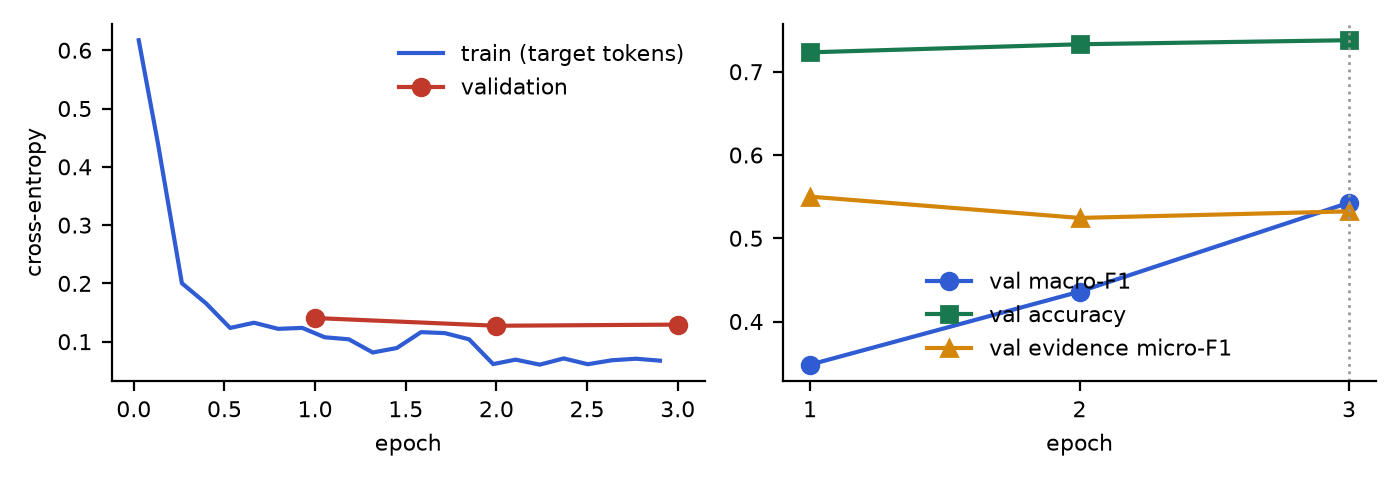
\includegraphics[width=\linewidth]{training_curves.png}
\caption{Training loss per optimiser step, and validation loss and generated-output validation macro-F1 per
epoch.}
\label{fig:training}
\end{figure}

\subsection{Classification: Before vs.\ After Fine-Tuning}
\begin{table*}[t]
\centering
\footnotesize
\caption{Same model before and after fine-tuning on identical examples (greedy, KV-cached decoder, bf16, max 64 new tokens). Macro-F1 over all 6 labels; MF1$_p$ over labels present in gold; Inc./Exc. = 4-label macro-F1 per criterion type; Ev = evidence F1; Inv = \% unparseable outputs.}
\label{tab:main}
\begin{tabular}{lrrrrrrrr}
\toprule
Model / split & Acc & MF1 & MF1$_p$ & Inc. & Exc. & Ev$_\mu$ & Ev$_M$ & Inv \\
\midrule
Base (zero-shot), val & 0.189 & 0.145 & 0.145 & 0.243 & 0.030 & 0.175 & 0.304 & 0.0 \\
Fine-tuned, val & 0.738 & 0.543 & 0.543 & 0.383 & 0.520 & 0.532 & 0.731 & 0.0 \\
\textbf{Base (zero-shot), test} & 0.160 & 0.129 & 0.155 & 0.207 & 0.042 & 0.169 & 0.354 & 0.0 \\
\textbf{Fine-tuned, test} & 0.733 & 0.440 & 0.528 & 0.425 & 0.299 & 0.561 & 0.819 & 0.0 \\
\bottomrule
\end{tabular}
\end{table*}

Table~\ref{tab:main} compares the same network with and without the adapter on identical inputs, using the
same prompt, decoder and parser. On the held-out test patients, test accuracy rose from 0.160 to 0.733
(patient-level bootstrap 95\% CI \ciacc). Macro-F1 over the labels present in gold rose from 0.155 to 0.528
(CI \cimf). Neither model produced an unparseable output, so the gain comes from label and evidence decisions,
not from formatting. The zero-shot base mostly answers \emph{included} or \emph{not applicable} and almost
never \emph{not enough information}: it treats absent facts as decisive.

Six-label macro-F1 on test (0.440) is lower than on validation (0.543) mainly because the test split contains
no \emph{excluded} example, which scores that class as~0. Over the labels present in gold the two splits agree
(0.528 vs.\ 0.543).

\begin{table}[t]
\centering
\footnotesize
\caption{Per-class results on the held-out test split (fine-tuned; base F1 for reference). Classes with zero support cannot be scored.}
\label{tab:perclass}
\begin{tabular}{llrrrrr}
\toprule
Type & Label & n & F1$_{base}$ & P & R & F1 \\
\midrule
inc. & included & 27 & 0.591 & 1.000 & 0.778 & 0.875 \\
inc. & not included & 7 & 0.000 & 0.000 & 0.000 & 0.000 \\
inc. & not enough information & 38 & 0.000 & 0.704 & 1.000 & 0.826 \\
inc. & not applicable & 3 & 0.235 & 0.000 & 0.000 & 0.000 \\
exc. & excluded & 0 & 0.000 & 0.000 & 0.000 & 0.000 \\
exc. & not excluded & 91 & 0.000 & 0.706 & 0.978 & 0.820 \\
exc. & not enough information & 28 & 0.000 & 0.000 & 0.000 & 0.000 \\
exc. & not applicable & 12 & 0.167 & 0.750 & 0.250 & 0.375 \\
\bottomrule
\end{tabular}
\end{table}

Per class (Table~\ref{tab:perclass}), the model is strong and precise on \emph{included} (P\,=\,1.00, F1 0.875)
and \emph{not excluded} (F1 0.820). It is weak on the rare classes:
\begin{itemize}
\item \emph{not included}: all 7 test cases were predicted \emph{not enough information};
\item \emph{not applicable}: recall is 0.20.
\end{itemize}
These are the classes with the fewest training examples, so the result matches the label skew documented in
Section~\ref{sec:split}. For exclusion criteria, 28 of the 66 \emph{not enough information} cases were
predicted \emph{not excluded}. This reproduces, in a milder form, the base model's habit of reading silence as
a negative finding. The confusion matrices in Fig.~\ref{fig:cm} show the same pattern.

\begin{figure}[t]
\centering
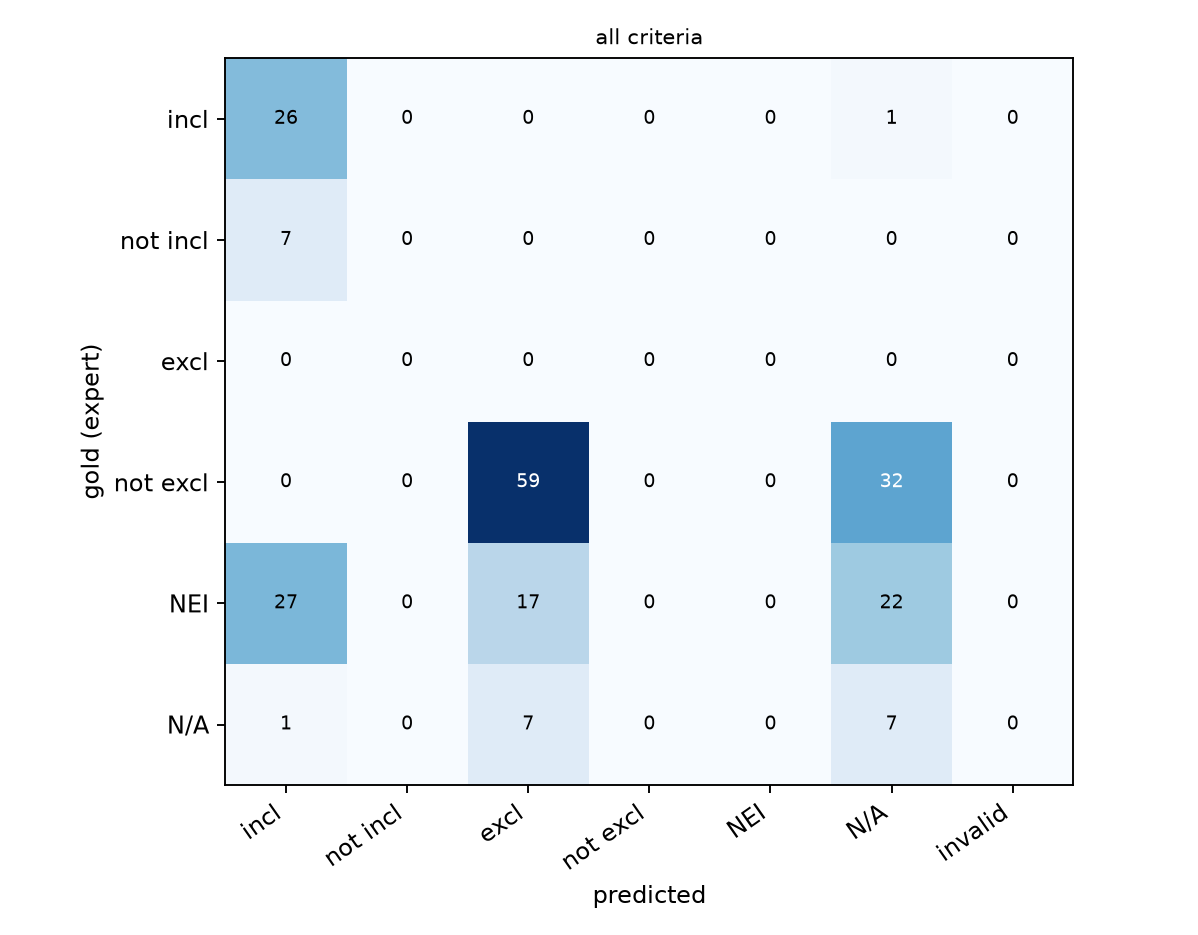
\includegraphics[width=0.49\linewidth]{cm_base_all.png}\hfill
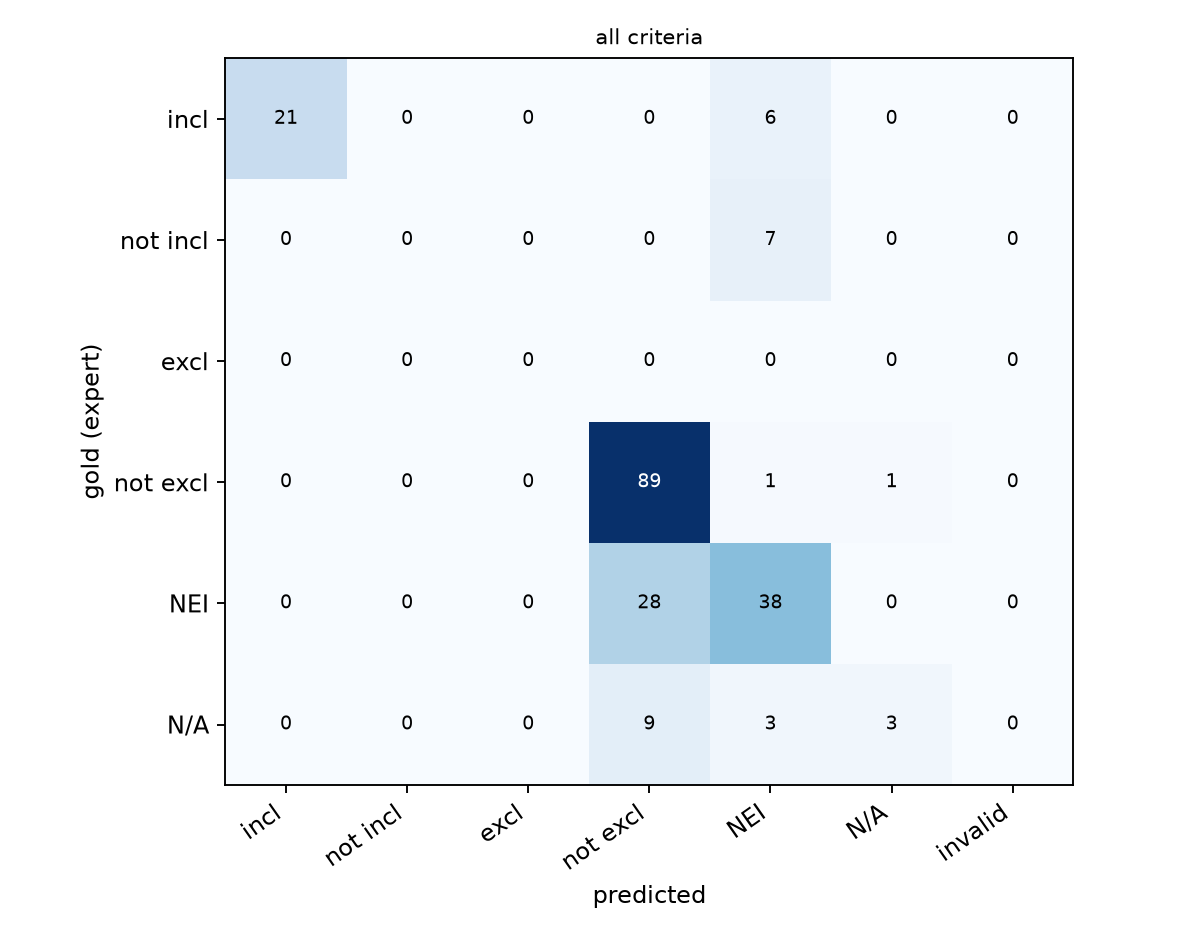
\includegraphics[width=0.49\linewidth]{cm_finetuned_all.png}
\caption{Test confusion matrices over all six labels: zero-shot base (left) and fine-tuned (right).}
\label{fig:cm}
\end{figure}

\subsection{Evidence Retrieval}
\begin{table*}[t]
\centering
\footnotesize
\caption{Evidence-sentence retrieval on the test split. Micro pools TP/FP/FN; macro averages per record (both-empty = 1, see Sec.~\ref{sec:metrics}). NE = non-empty-gold subset; Abst. = correct empty predictions for empty gold; Uns. = cited IDs not in the note.}
\label{tab:evidence}
\begin{tabular}{lrrrrrrrrr}
\toprule
Model & P$_\mu$ & R$_\mu$ & F1$_\mu$ & P$_M$ & R$_M$ & F1$_M$ & F1$_{NE}$ & Abst. & Uns. \\
\midrule
Base & 0.097 & 0.649 & 0.169 & 0.374 & 0.899 & 0.354 & 0.374 & 53/145 & 0 \\
Fine-tuned & 0.500 & 0.638 & 0.561 & 0.888 & 0.904 & 0.819 & 0.663 & 131/145 & 0 \\
\bottomrule
\end{tabular}
\end{table*}

Fine-tuning improves evidence citation more than any other metric (Table~\ref{tab:evidence}). Micro-F1 rose
from 0.169 to 0.561, and the gain came almost entirely from precision (0.097 to 0.500), with recall unchanged
(0.649 vs.\ 0.638). The base model cites many sentences indiscriminately. The fine-tuned model abstains
correctly on 131 of the 145 empty-gold criteria, compared with 53 for the base model. On the non-empty-gold
subset, which isolates retrieval from abstention, F1 rose from 0.374 to 0.663. Neither model cited a sentence
ID outside the note.

\begin{figure*}[t]
\centering
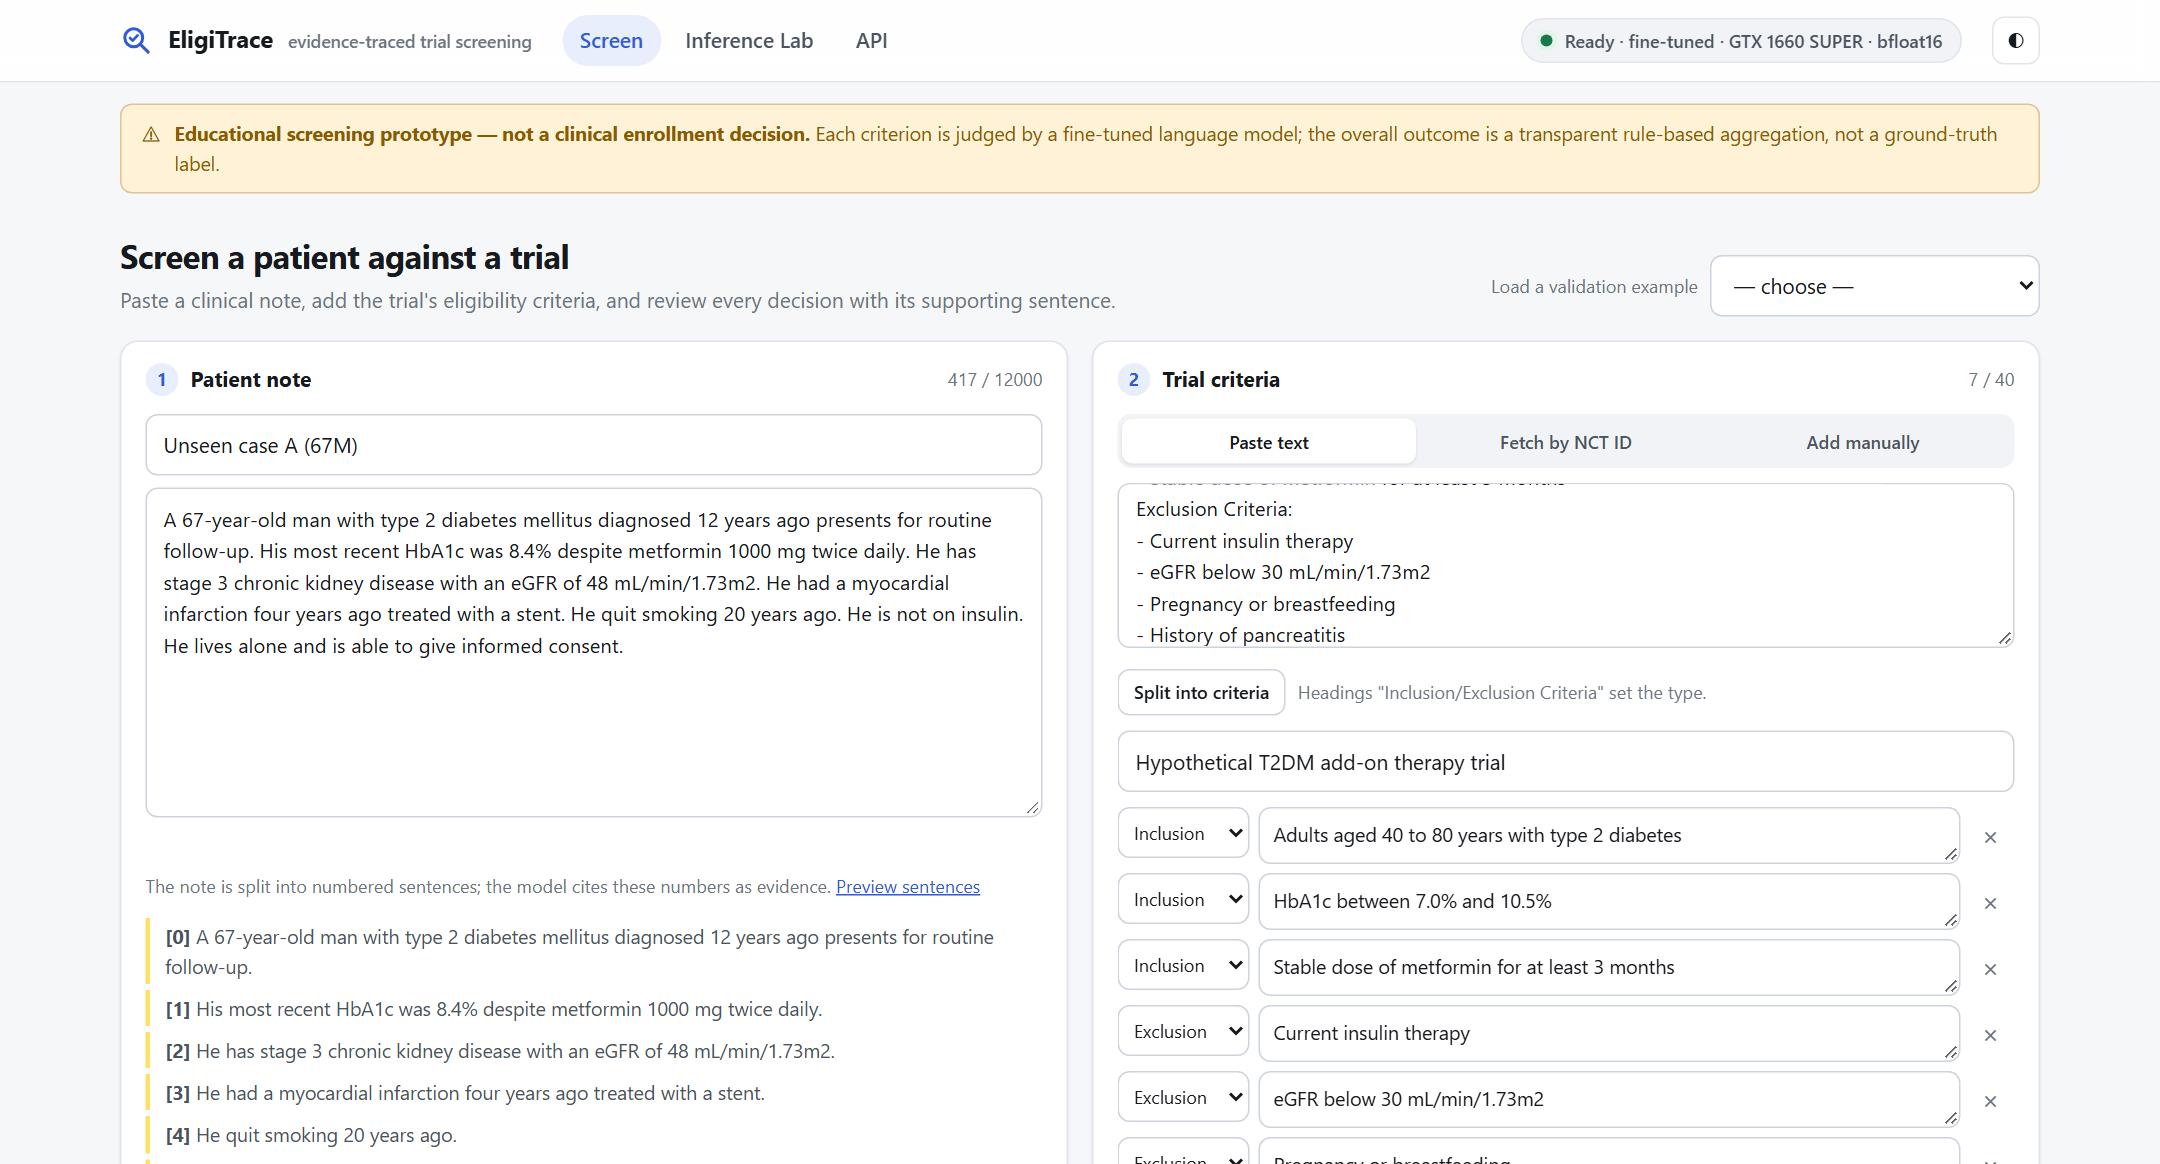
\includegraphics[width=0.49\linewidth]{screens/02_input_top.png}\hfill
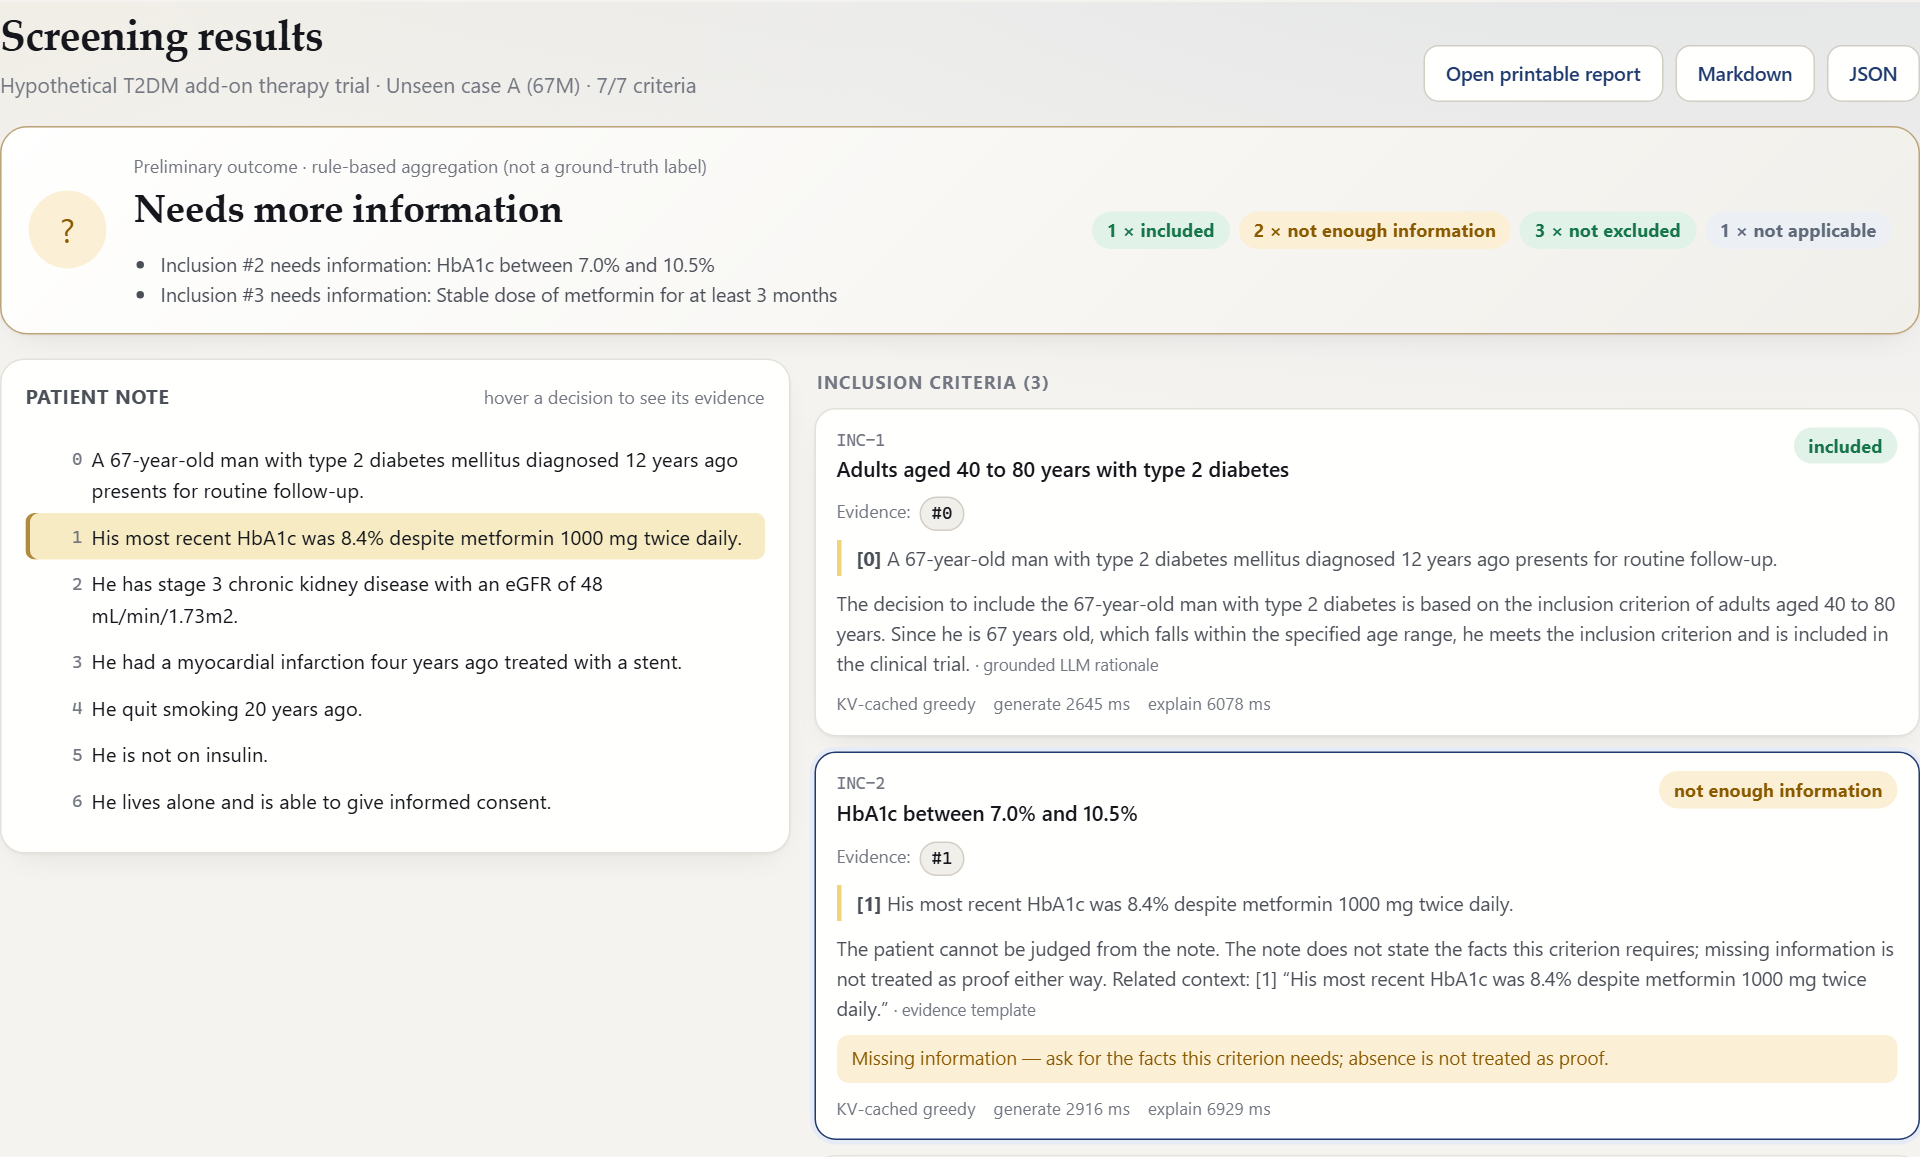
\includegraphics[width=0.49\linewidth]{screens/03_results_top.png}\\[4pt]
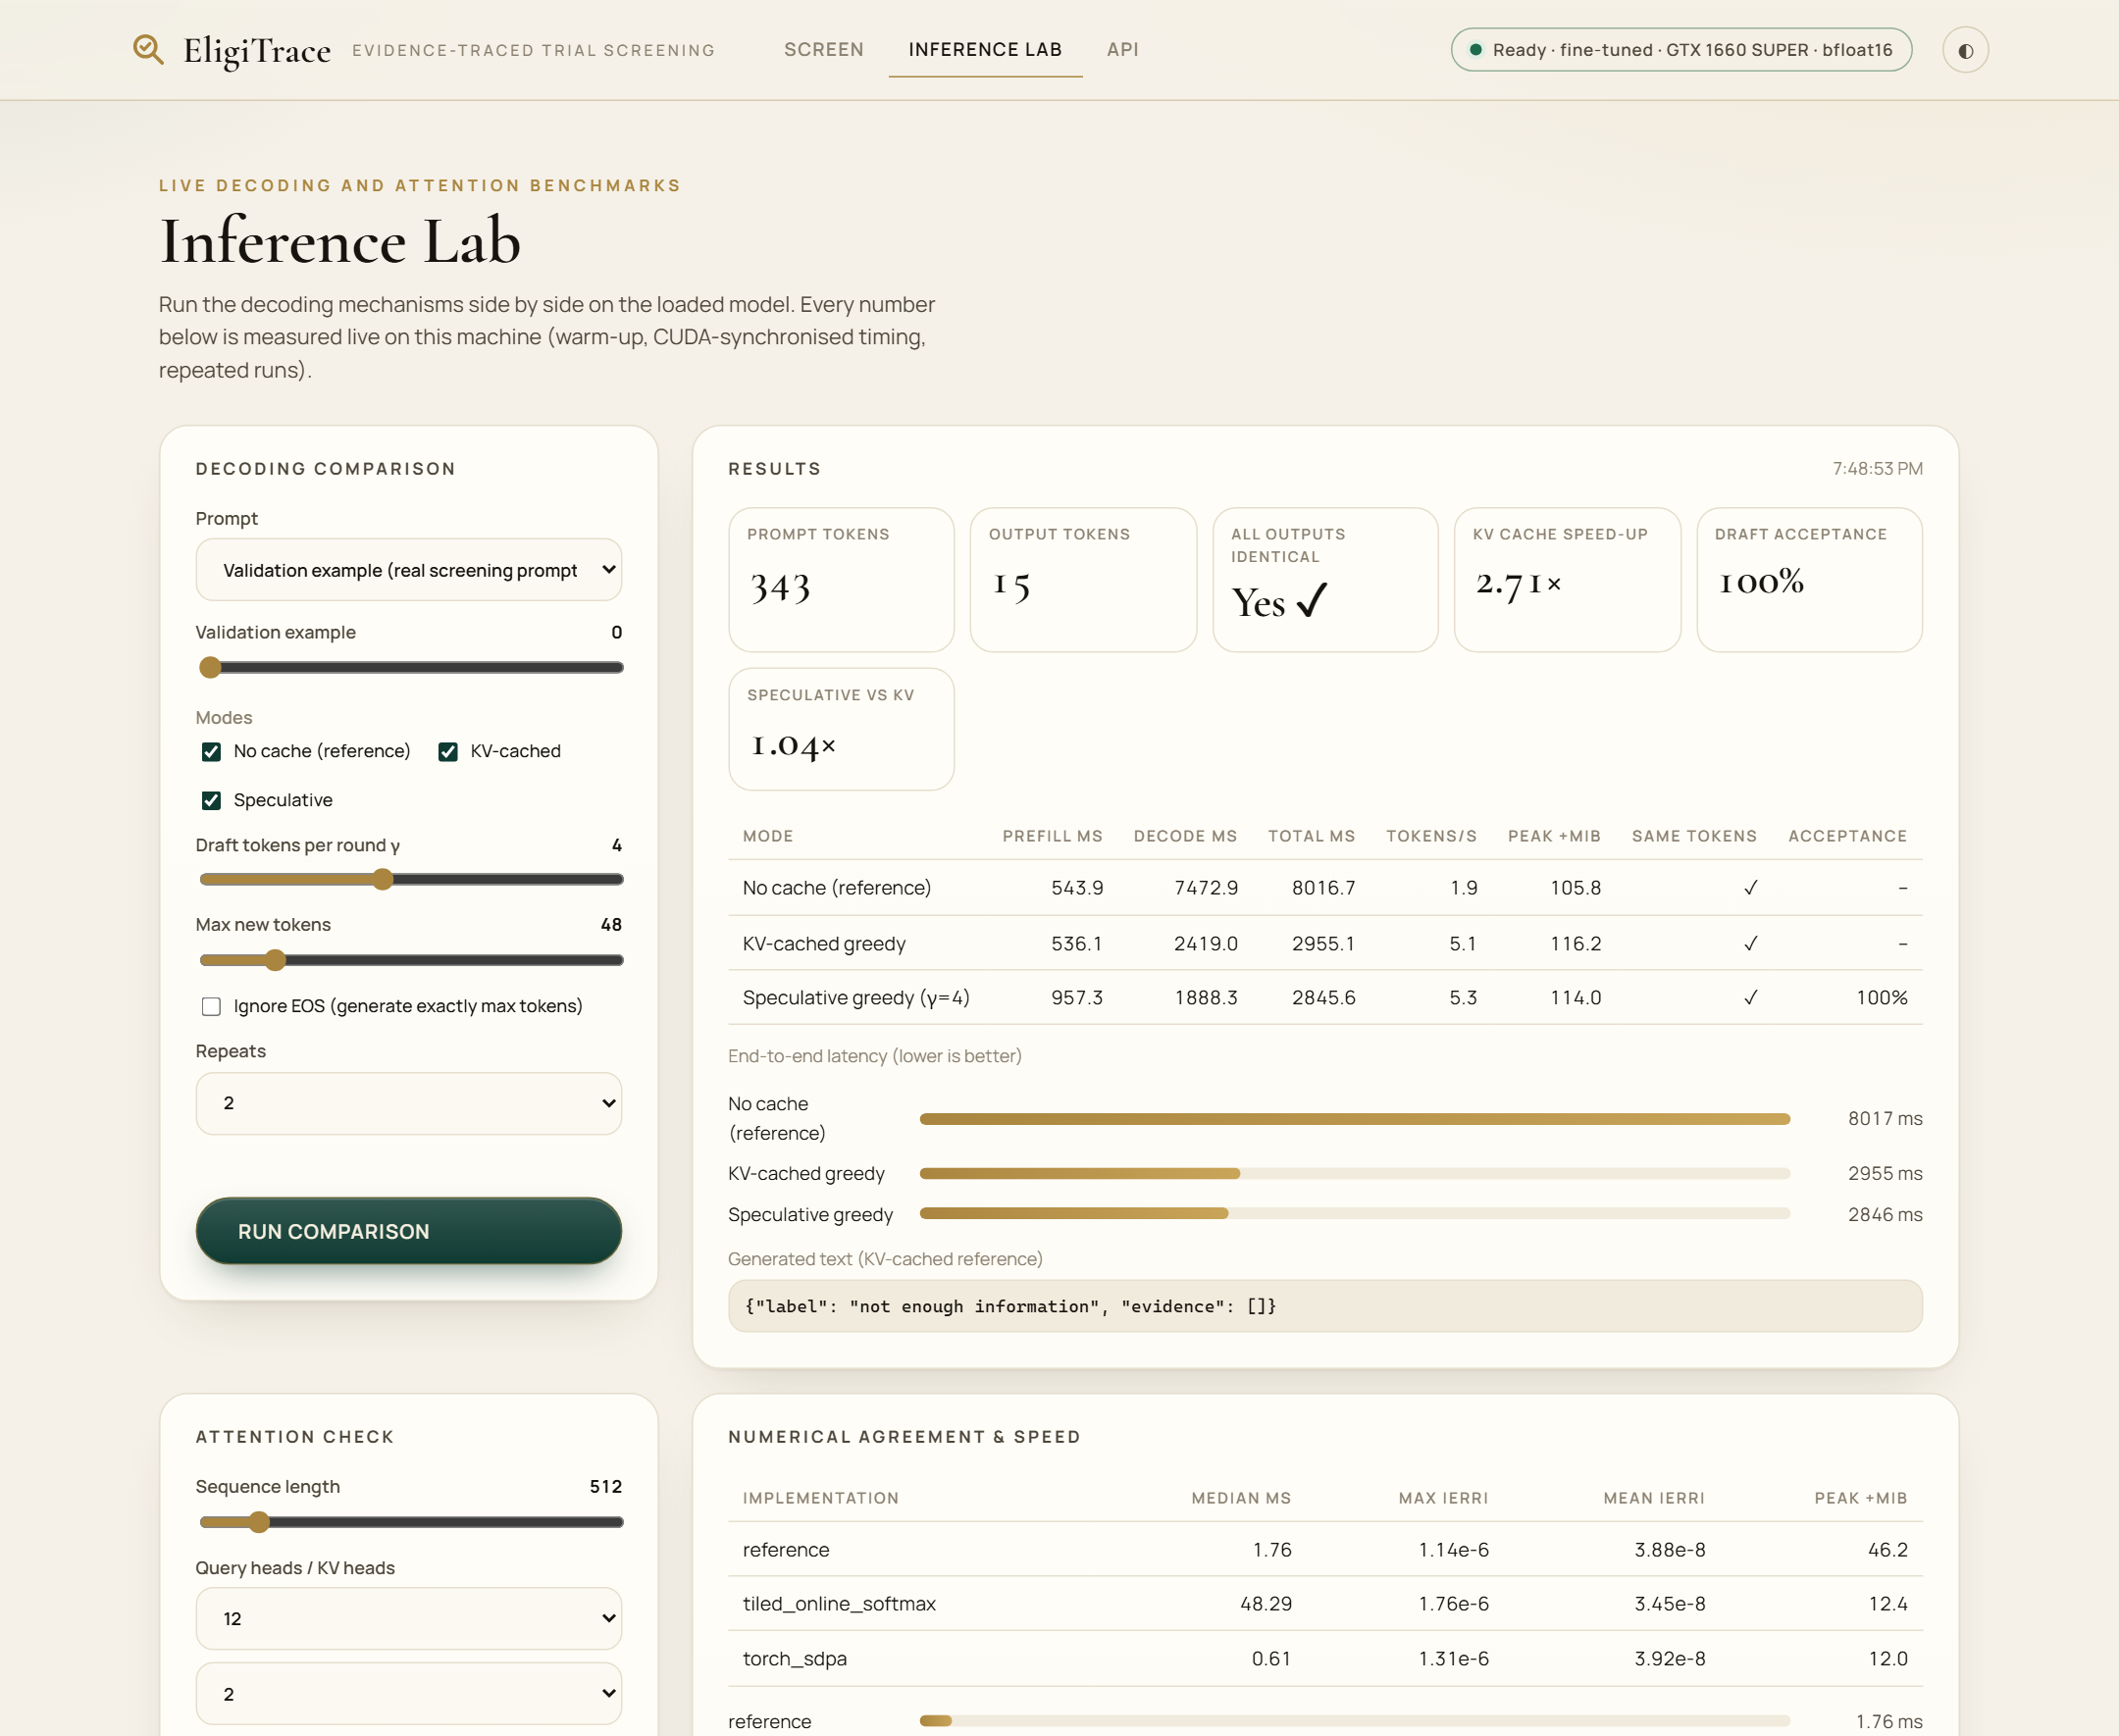
\includegraphics[width=0.49\linewidth]{screens/06_lab.png}\hfill
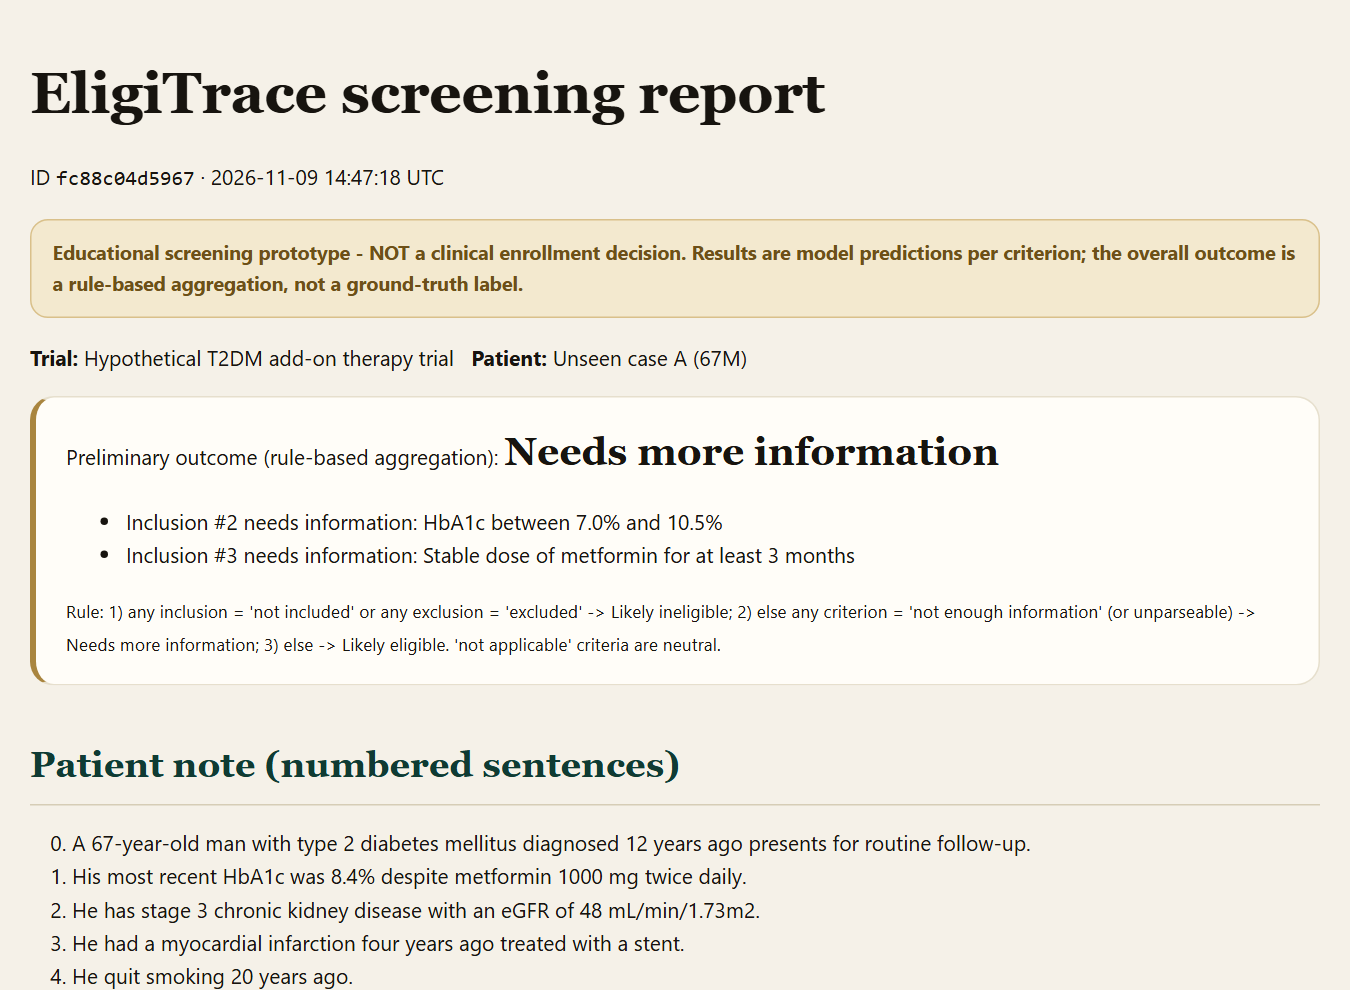
\includegraphics[width=0.49\linewidth]{screens/04_report_top.png}
\caption{\sys\ application. Top: input of an unseen note and criteria (left), and criterion results with
highlighted evidence, grounded rationales and the rule-based outcome (right). Bottom: Inference Lab with live
decoder and attention comparisons (left), and the exported report with provenance (right).}
\label{fig:app}
\end{figure*}

\subsection{Error Analysis}
\begin{table}[t]
\centering
\footnotesize
\caption{Rule-assigned error categories, fine-tuned model, test split (55 wrong labels of 206; one error may have several).}
\label{tab:errors}
\begin{tabular}{lr}
\toprule
Category & Count \\
\midrule
correct label, wrong evidence & 34 \\
missing information treated as decisive (unsupported decision) & 28 \\
temporal qualifier & 19 \\
false 'not enough information' (evidence was present) & 17 \\
not-applicable confusion & 13 \\
negation in evidence & 7 \\
numeric / threshold reasoning & 6 \\
cited evidence where experts found none & 3 \\
\bottomrule
\end{tabular}
\end{table}

Of the 206 test criteria, 55 received the wrong label. Table~\ref{tab:errors} groups them with deterministic
rules (\texttt{evaluation/errors.py}). The most frequent pattern is an unsupported decision, where missing
information is treated as decisive (28 cases). Temporal qualifiers such as ``within the past 6 months'' and
``history of'' are next (19 cases). The opposite error, answering \emph{not enough information} although the
experts found the note sufficient, occurs 17 times.

One instructive case is a vascular-surgery trial whose inclusion criteria list specific operations
(``patients undergoing open abdominal aortic aneurysm repair''). For a patient with a femoral pseudoaneurysm,
the experts labelled these criteria \emph{not included} with no evidence: a note that describes a different
procedure implies the listed one is not happening. The model answered \emph{not enough information} and cited
the three sentences describing the actual procedure. Expert reasoning of this kind rests on the absence of a
fact in an otherwise complete clinical picture, and it is underrepresented in 603 training examples.

A further 34 records have the correct label but differ from the gold evidence. Most of these are omissions on
\emph{not excluded} criteria, where the annotators cited background sentences such as the demographic opening
line.

\subsection{KV-Cached Decoding}\label{sec:res-kv}
\begin{table*}[t]
\centering
\footnotesize
\caption{KV-cached vs.\ no-cache greedy decoding (fine-tuned target, bf16, batch 1, EOS disabled; mean of 3 synchronised runs after 1 warm-up). Peak = extra MiB over resident weights. Eq. = token-identical output.}
\label{tab:kv}
\begin{tabular}{rrrrrrrrrrc}
\toprule
In & Out & Pre ms & Dec ms & tok/s & Dec ms$_{nc}$ & tok/s$_{nc}$ & Speed-up & Peak & Peak$_{nc}$ & Eq. \\
\midrule
128 & 16 & 189 & 1098 & 12.4 & 3810 & 4.0 & 3.5 & 44 & 42 & no@5 \\
128 & 64 & 216 & 4546 & 13.4 & 16357 & 3.9 & 3.6 & 44 & 57 & no@5 \\
128 & 128 & 228 & 10014 & 12.5 & 38493 & 3.3 & 3.8 & 44 & 75 & no@5 \\
512 & 16 & 653 & 1084 & 9.2 & 10882 & 1.4 & 10.0 & 172 & 154 & yes \\
512 & 64 & 667 & 4570 & 12.2 & 45849 & 1.4 & 10.0 & 172 & 168 & yes \\
512 & 128 & 683 & 9163 & 13.0 & 98547 & 1.3 & 10.8 & 172 & 188 & yes \\
1024 & 16 & 1380 & 1151 & 6.3 & 21827 & 0.7 & 19.0 & 346 & 305 & yes \\
1024 & 64 & 1382 & 5026 & 10.0 & 89785 & 0.7 & 17.9 & 346 & 319 & yes \\
1024 & 128 & 1352 & 9326 & 12.0 & 186221 & 0.7 & 20.0 & 346 & 337 & no@84 \\
\bottomrule
\end{tabular}
\end{table*}

Table~\ref{tab:kv} and Fig.~\ref{fig:kv} compare the two decoders. Prefill cost is the same for both, since
both process the prompt once. Without a cache, every decode step reprocesses the whole sequence, so no-cache
throughput falls from 4.0 to 0.7\,tok/s as the input grows from 128 to 1024 tokens. With the cache, each step
costs one token through the network and throughput stays between 9 and 13\,tok/s. Decode speed-up therefore
grows with context: about $3.6\times$ at 128 input tokens, $10\times$ at 512 and $18$--$20\times$ at 1024.

Peak extra memory is dominated by prefill activations (the $T\times151{,}936$ logit matrix), not by the cache.
The cache adds 28\,KiB per token, so it occupies only 32\,MiB even at 1{,}152 tokens. At batch~1 on this GPU,
decoding is launch-bound: a single-token step costs about 75--110\,ms whatever the context length, which is
why the cached throughput stays flat.

\begin{figure}[t]
\centering
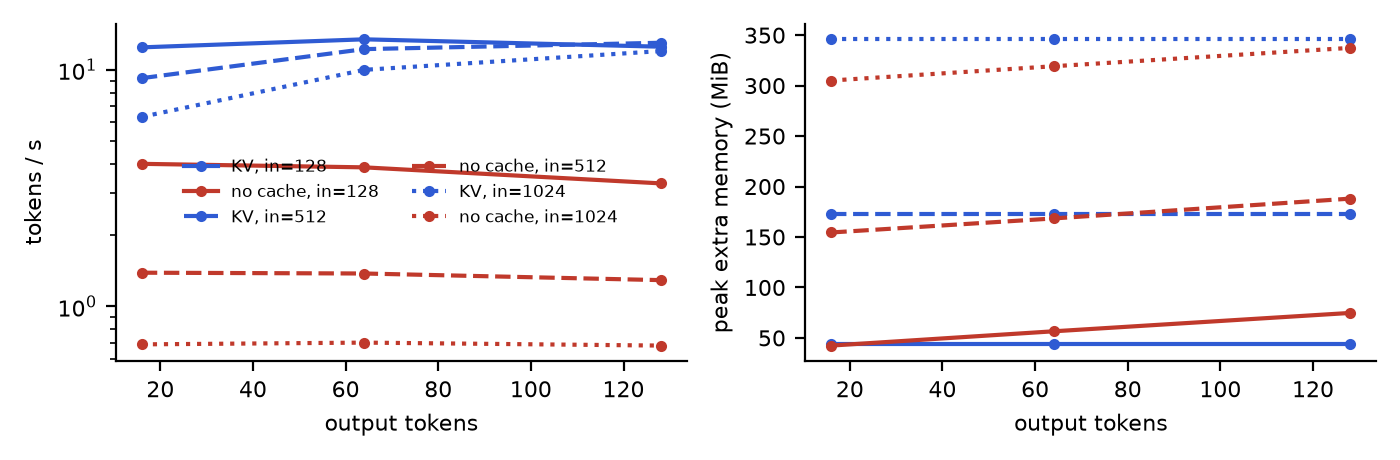
\includegraphics[width=\linewidth]{kv_benchmark.png}
\caption{Decode throughput (left) and peak extra memory (right) of the KV-cached decoder and the no-cache reference vs.\ input and output length.}
\label{fig:kv}
\end{figure}

\textbf{Equality.} The CPU fp64 tests on tiny Qwen2 models and the bf16 GPU test on the base model produce
token-identical output for both decoders. With the merged fine-tuned weights in bf16, 6 of the 9 benchmark
cases are identical. The other three diverge at a step where the top-2 logit margin is 0.125, which is exactly
one bf16 unit in the last place for logits between 16 and 32. In other words, the two candidate tokens are
tied at bf16 resolution. The cached path computes attention for one query against stored keys, while the
reference recomputes the full $T\times T$ product; the two reduction orders round differently, and a tie can
go either way. Section~\ref{sec:res-numerics} tests this explanation in fp32.

\subsection{Tiled Attention}
\begin{table}[t]
\centering
\footnotesize
\caption{Attention agreement with a float64 reference over the validation grid (3 head layouts incl.\ GQA 12:2, 8 $(S_q,S_k)$ shapes incl.\ decode $S_q{=}1$, $d\in\{32,64,128\}$, causal on/off; tiled also over tile sizes 16/64/128).}
\label{tab:attnerr}
\begin{tabular}{llrrr}
\toprule
Impl. & dtype & Cases & max $|\Delta|$ & mean $|\Delta|$ \\
\midrule
reference & bfloat16 & 144 & 7.80e-03 & 1.83e-04 \\
reference & float16 & 144 & 9.76e-04 & 2.28e-05 \\
reference & float32 & 144 & 0.00e+00 & 0.00e+00 \\
tiled & bfloat16 & 432 & 7.80e-03 & 1.83e-04 \\
tiled & float16 & 432 & 9.76e-04 & 2.28e-05 \\
tiled & float32 & 432 & 2.74e-06 & 2.82e-08 \\
torch\_sdpa & bfloat16 & 144 & 7.80e-03 & 1.83e-04 \\
torch\_sdpa & float16 & 144 & 9.76e-04 & 2.28e-05 \\
torch\_sdpa & float32 & 144 & 2.38e-06 & 2.63e-08 \\
\bottomrule
\end{tabular}
\end{table}

Against a float64 ground truth, the tiled kernel matches PyTorch SDPA to the precision of its storage format
(Table~\ref{tab:attnerr}). In fp32 its maximum error is $2.7\times10^{-6}$ against $2.4\times10^{-6}$ for SDPA,
over 432 cases that cover GQA (12:2), decode shapes with $S_q{=}1$, causal and non-causal masks, and tile sizes
16, 64 and 128. In bf16 and fp16 all three implementations have the same error, set by rounding the output to
the storage type.

Speed and memory show the expected trade-off (Fig.~\ref{fig:attn}). On the GTX~1660 SUPER (sm\_75), PyTorch's
fused flash and memory-efficient kernels are unavailable in bf16, so the fair baseline is the unfused
\texttt{math} backend. At sequence length 4096, that backend materialises the score matrix and needs 1.9\,GB of
extra memory, whereas the tiled kernel needs 41\,MiB, about 46$\times$ less. Being a Python loop over tiles, the
tiled kernel is slower: 465\,ms vs.\ 73\,ms with 128-wide tiles. Larger tiles reduce the number of kernel
launches and run $3.7\times$ faster than 64-wide tiles. This is the I/O-versus-launch trade-off that fused
kernels such as FlashAttention remove~\cite{dao2022flashattention}.

\begin{figure}[t]
\centering
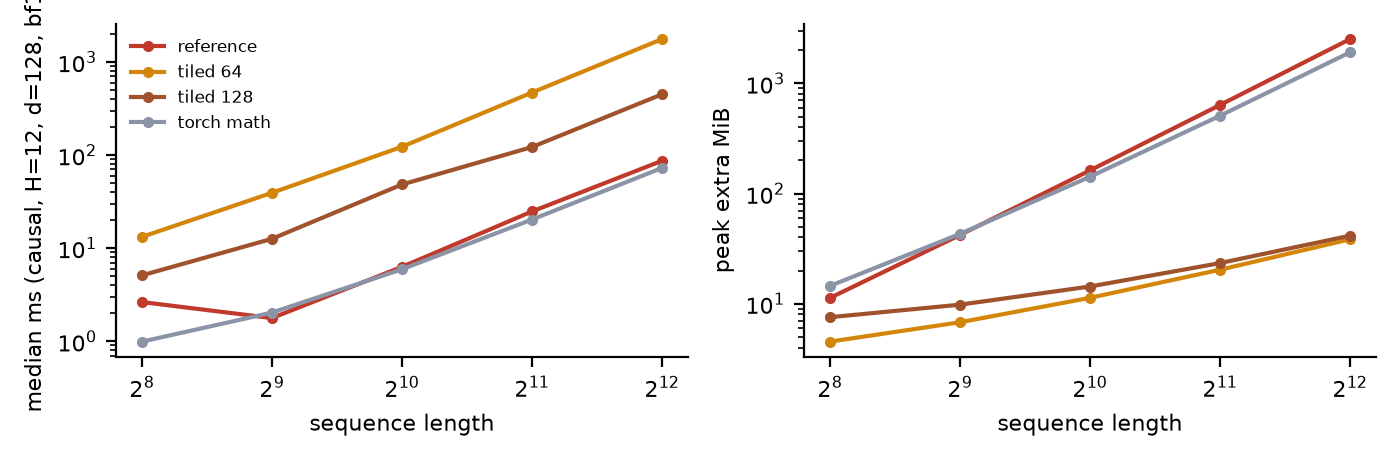
\includegraphics[width=\linewidth]{attention_benchmark.png}
\caption{Attention latency and peak extra memory vs.\ sequence length (bf16, GPU, 12 query / 2 KV heads,
$d$=128, causal).}
\label{fig:attn}
\end{figure}

\subsection{Speculative Decoding}
\begin{table*}[t]
\centering
\footnotesize
\caption{Greedy speculative decoding (target: fine-tuned Qwen2.5-1.5B, draft: Qwen2.5-0.5B, bf16) vs.\ KV-cached greedy on the same 8 validation prompts. Acc.\ = accepted/proposed; $\bar n$ = accepted per round; Fwd/tok = target forwards per output token.}
\label{tab:spec}
\begin{tabular}{lrrrrrrrc}
\toprule
Workload & $\gamma$ & Lat. ms & tok/s & Acc. & $\bar n$ & Fwd/tok & Speed-up & Eq. \\
\midrule
task\_json & greedy & 1437 & 9.9 & -- & -- & 1.00 & 1.00 & yes \\
task\_json & 1 & 2089 & 6.8 & 0.91 & 0.91 & 0.58 & 0.69 & yes \\
task\_json & 2 & 2190 & 6.5 & 0.71 & 1.43 & 0.48 & 0.66 & yes \\
task\_json & 3 & 2296 & 6.3 & 0.60 & 1.80 & 0.43 & 0.63 & no \\
task\_json & 4 & 2279 & 6.3 & 0.59 & 2.35 & 0.37 & 0.63 & yes \\
task\_json & 6 & 2420 & 5.9 & 0.51 & 3.04 & 0.32 & 0.59 & yes \\
task\_json & 8 & 2767 & 5.1 & 0.40 & 3.22 & 0.31 & 0.52 & yes \\
free\_96 & greedy & 7345 & 13.1 & -- & -- & 1.00 & 1.00 & yes \\
free\_96 & 1 & 11392 & 8.4 & 0.76 & 0.76 & 0.58 & 0.64 & no \\
free\_96 & 2 & 11730 & 8.2 & 0.61 & 1.21 & 0.46 & 0.63 & no \\
free\_96 & 3 & 12251 & 7.8 & 0.55 & 1.62 & 0.39 & 0.60 & no \\
free\_96 & 4 & 13105 & 7.3 & 0.48 & 1.90 & 0.35 & 0.56 & no \\
free\_96 & 6 & 13899 & 6.9 & 0.44 & 2.59 & 0.29 & 0.53 & no \\
free\_96 & 8 & 18911 & 5.1 & 0.29 & 2.25 & 0.32 & 0.39 & no \\
\bottomrule
\end{tabular}
\end{table*}

The draft and target models share tokenizer, special tokens and chat template, which we verified
programmatically. Acceptance is high: 91\% of drafted tokens are accepted at $\gamma{=}1$ on the
structured-output task, and acceptance falls to 40\% at $\gamma{=}8$ (Table~\ref{tab:spec}, Fig.~\ref{fig:spec}).
The number of target forwards per output token falls from 1.0 to 0.31.

Even so, speculative decoding was \emph{slower} than KV-cached greedy decoding at every $\gamma$, at
0.39--0.69$\times$ its speed. The reason is that at batch~1 on this GPU, forward cost scales with the number of
layers and kernel launches rather than with parameter count. The 0.5B draft has 24 layers against the target's
28, so a draft step costs almost as much as a target step. We timed this directly, with greedy cached decoding
after a 512-token prompt in bf16: one draft step took 189\,ms and one target step took 239\,ms, a ratio of
0.79, although the draft has a third of the target's parameters. Saving a target forward therefore saves less time
than the extra draft steps add. Speculative decoding pays off when the draft is much cheaper per token than the
target, for example a larger target, a shallower draft, or a compute-bound regime. We report the negative
result as measured.

\begin{figure}[t]
\centering
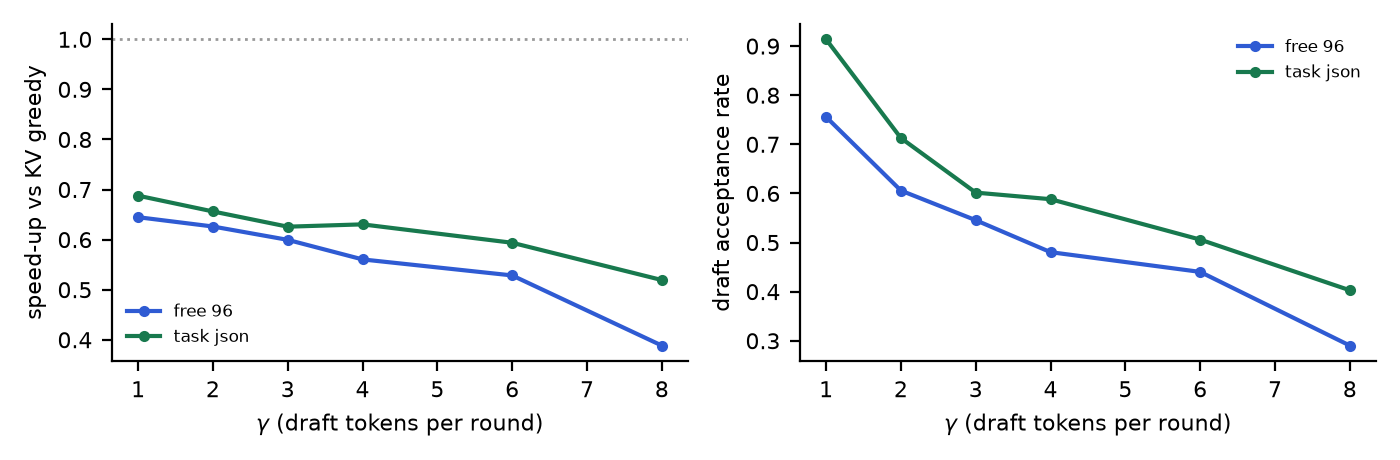
\includegraphics[width=\linewidth]{spec_benchmark.png}
\caption{Speculative decoding: acceptance rate and speed-up over KV-cached greedy decoding vs.\ draft length
$\gamma$.}
\label{fig:spec}
\end{figure}

\subsection{Numerical Agreement in bf16 vs.\ fp32}\label{sec:res-numerics}
All three mechanisms are exact in exact arithmetic, yet each produced a few bf16 outputs that differ from its
reference. We checked whether these differences come from bugs or from rounding, using
\texttt{speculative/investigate.py}, \texttt{attention/hf\_integration.py} and \texttt{kvcache/fp32\_check.py}.

\textbf{Margins at the divergence point.} Every bf16 divergence we found occurs where the two best logits
differ by at most 0.125. For logits in $[16,32)$, the spacing between adjacent bf16 values is $2^{4-7}=0.125$,
so the two tokens are tied, or one rounding step apart. For speculative example~0, the target logits at
step~22 are 18.375 vs.\ 18.25 when tokens are processed one at a time, as in greedy decoding. Inside the
5-token verification block used by speculative decoding, the same two logits come out \emph{exactly equal}
(17.875 and 17.875), and the tie is broken the other way. The single-token and block paths differ by up to 0.84
in individual logits. Different matrix shapes select different GEMM kernels and reduction orders, and bf16
keeps only 8 bits of mantissa.

\textbf{fp32 reruns.} Table~\ref{tab:fp32} repeats the diverging cases in fp32 on the CPU, without changing any
code. Speculative decoding then matches greedy decoding token for token on all three investigated prompts.
With the tiled kernel substituted for every attention layer of the fine-tuned model through the Transformers
\texttt{AttentionInterface}, final-position logits stay within $3.4\times10^{-4}$ of SDPA. Greedy output is
identical on all three prompts, whereas in bf16 the logit gap is 0.5--0.7 and one prompt diverges.
Finally, the KV-cached decoder matches the no-cache reference in fp32 on both bf16-diverging KV cases: (128 in,
16 out), which diverged at step~5, and (1024 in, 128 out), which diverged at step~84. The fp32 runs took
59\,min on the CPU, mostly in the quadratic no-cache reference.

\begin{table}[t]
\centering
\footnotesize
\caption{Token agreement with the reference in bf16 (GPU) vs.\ fp32 (CPU), on the cases that diverged in
bf16.}
\label{tab:fp32}
\begin{tabular}{lcc}
\toprule
Check & bf16 GPU & fp32 CPU \\
\midrule
Speculative vs.\ greedy ($\gamma{=}4$, 3 prompts) & 1/3 equal & 3/3 equal \\
Tiled attention in model vs.\ SDPA (3 prompts) & 2/3 equal & 3/3 equal \\
\quad max $|\Delta\text{logit}|$ & 0.70 & $3.4\times10^{-4}$ \\
KV-cached vs.\ no-cache (2 diverging cases) & 0/2 equal & 2/2 equal \\
\bottomrule
\end{tabular}
\end{table}

The mechanisms are therefore exact. In bf16 they are reproducible only up to ties within one rounding step,
which is also true of production inference stacks. Any bf16 equality claim should be read with that caveat.


\subsection{Application}\label{sec:res-app}
Fig.~\ref{fig:app} shows the running application, served on the same GPU used for evaluation. Each test used a
note that is not in the dataset, together with criteria that we wrote ourselves:
\begin{itemize}
\item a 67-year-old man with type~2 diabetes and stage~3 chronic kidney disease;
\item a hypothetical add-on therapy trial with three inclusion and four exclusion criteria.
\end{itemize}
The note is split into numbered sentences, and each criterion is decoded and displayed as soon as it finishes.
Each result card shows:
\begin{itemize}
\item the label, with both criterion types kept and all expert categories preserved;
\item the cited sentences, which are also highlighted in the note;
\item a rationale that passed the grounding check, or the deterministic template when it did not.
\end{itemize}
The overall outcome is shown together with the rule that produced it.

Invalid input is rejected with a field-level message and the user's draft is kept. This covers empty notes,
malformed NCT IDs and unknown labels. An unreachable ClinicalTrials.gov service or a model that is still
loading returns a clear message, not a stack trace.

The Inference Lab runs the no-cache, KV-cached and speculative decoders on the loaded model. For each run it
reports timing, token equality and draft acceptance, and it also runs the attention check against a float64
ground truth.

\begin{figure*}[t]
\centering
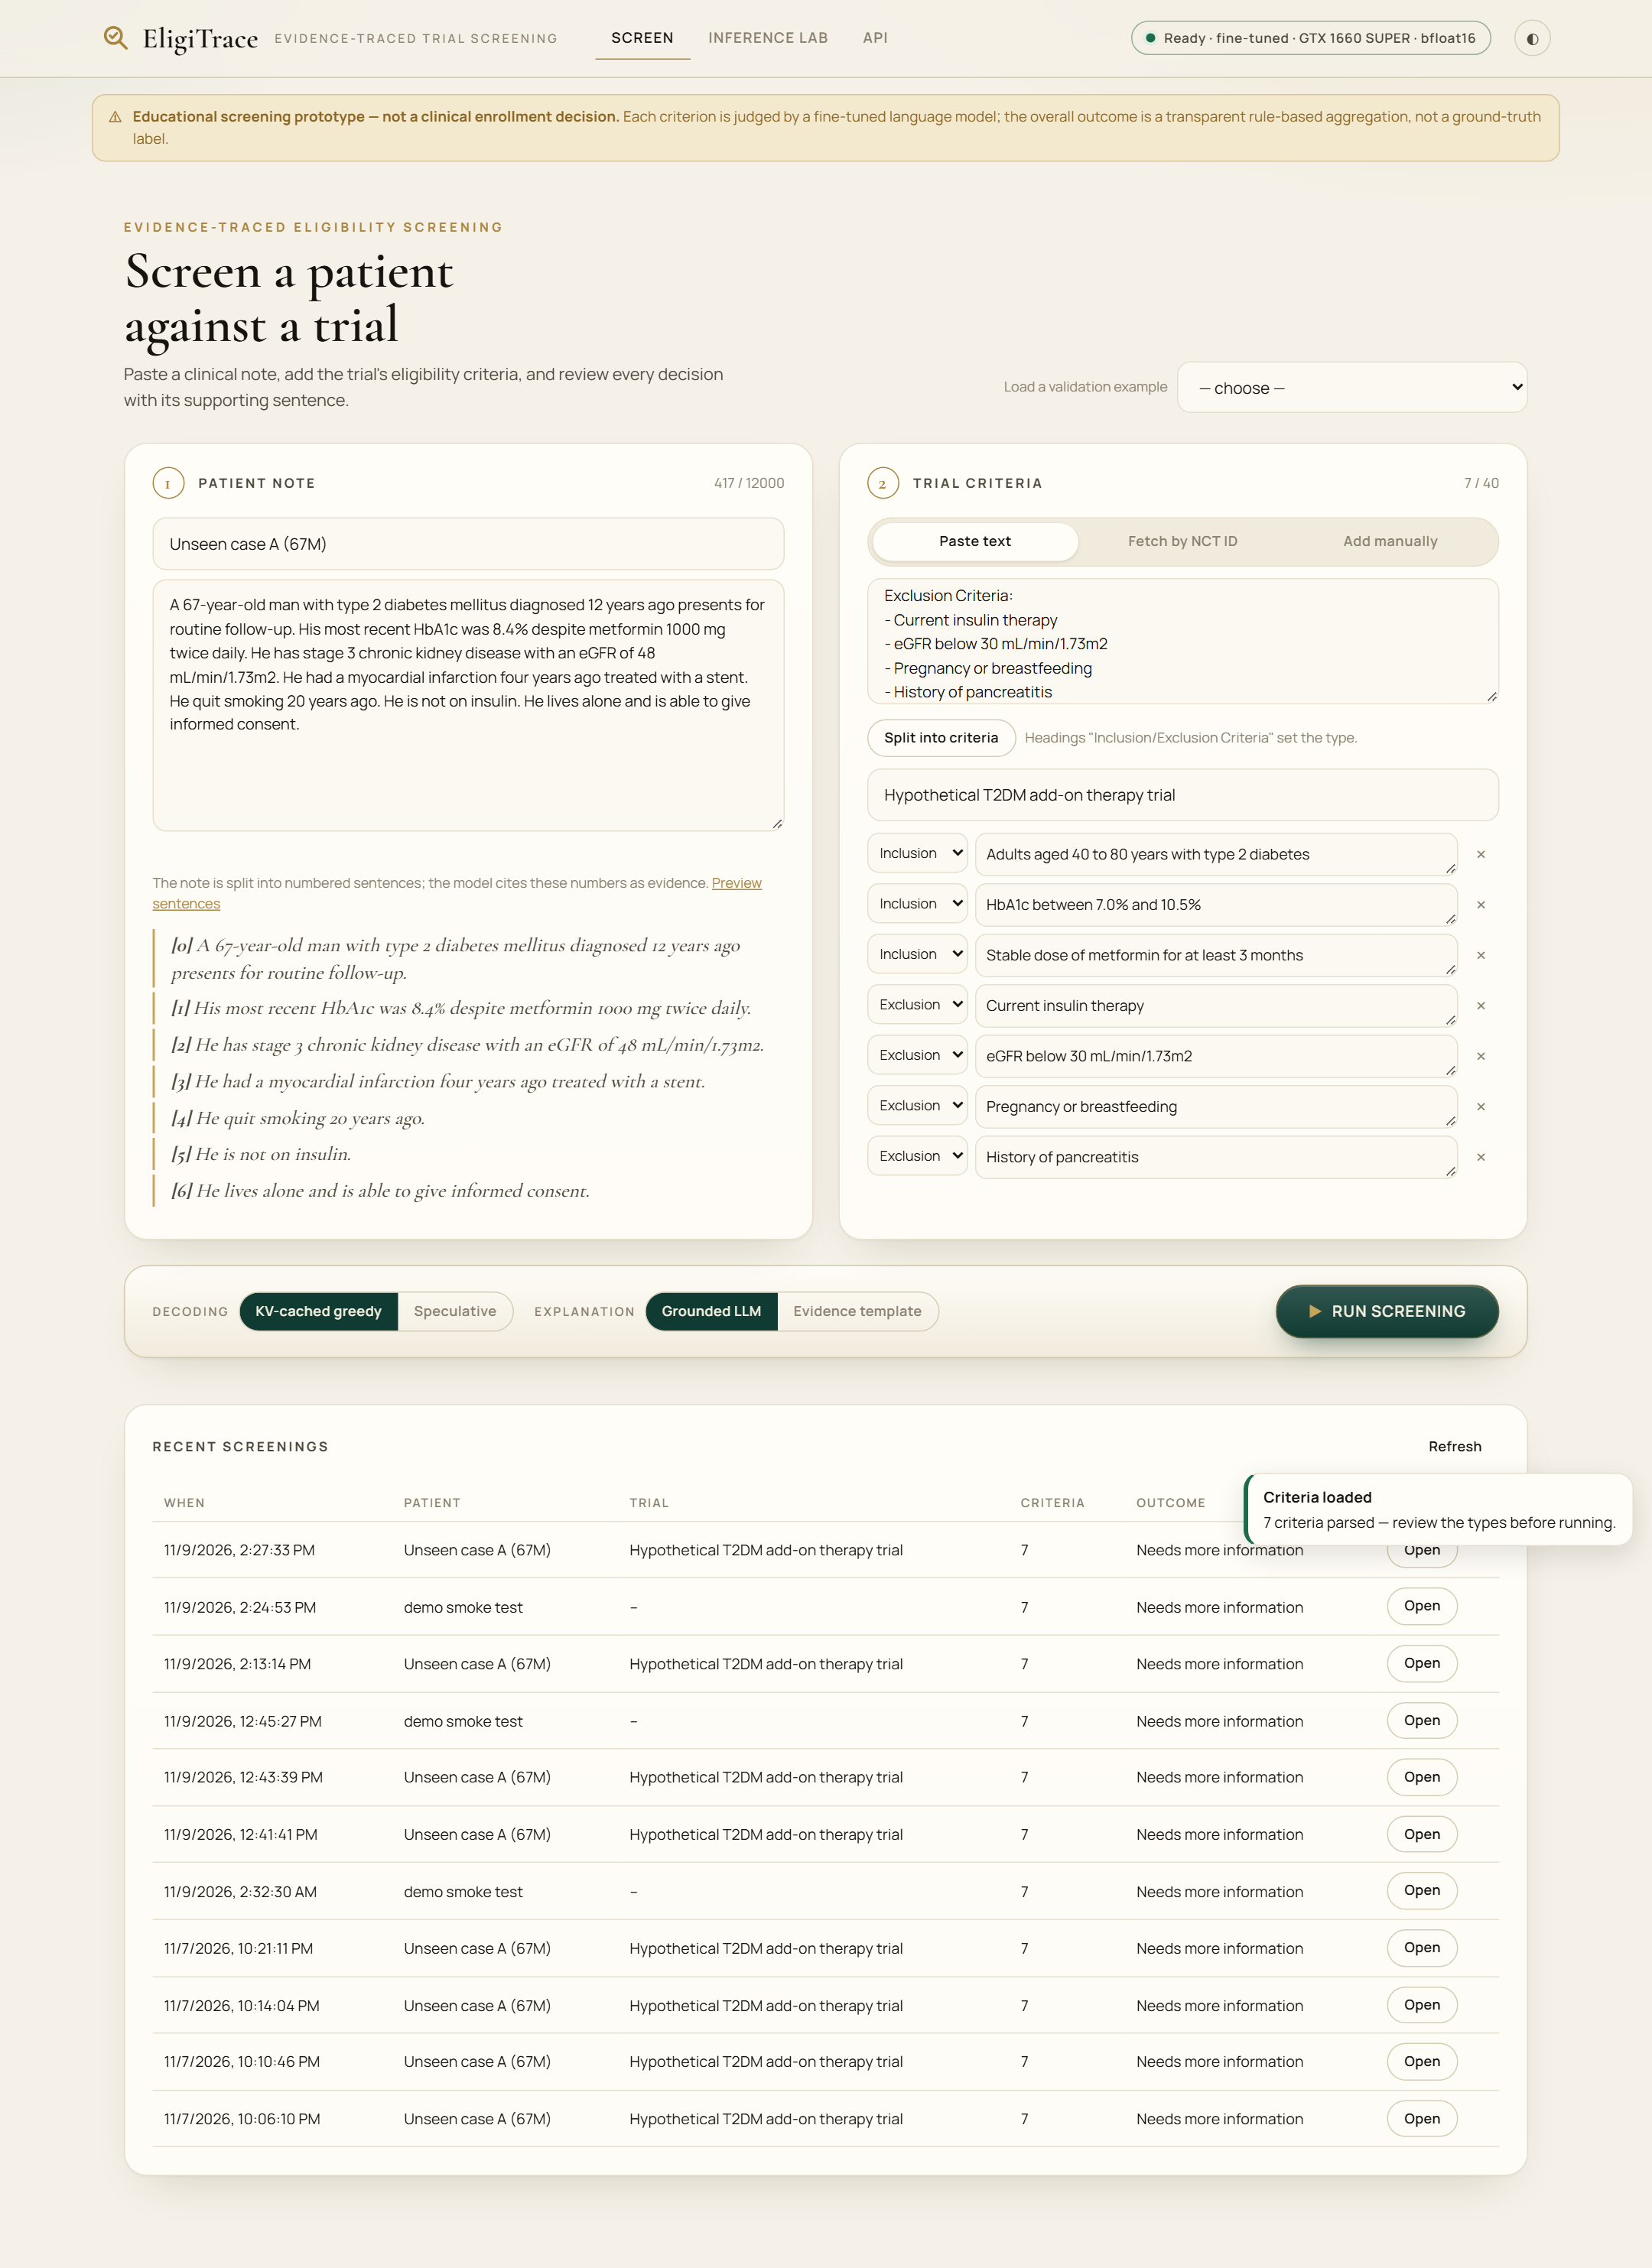
\includegraphics[width=0.49\linewidth]{screens/02_input.png}\hfill
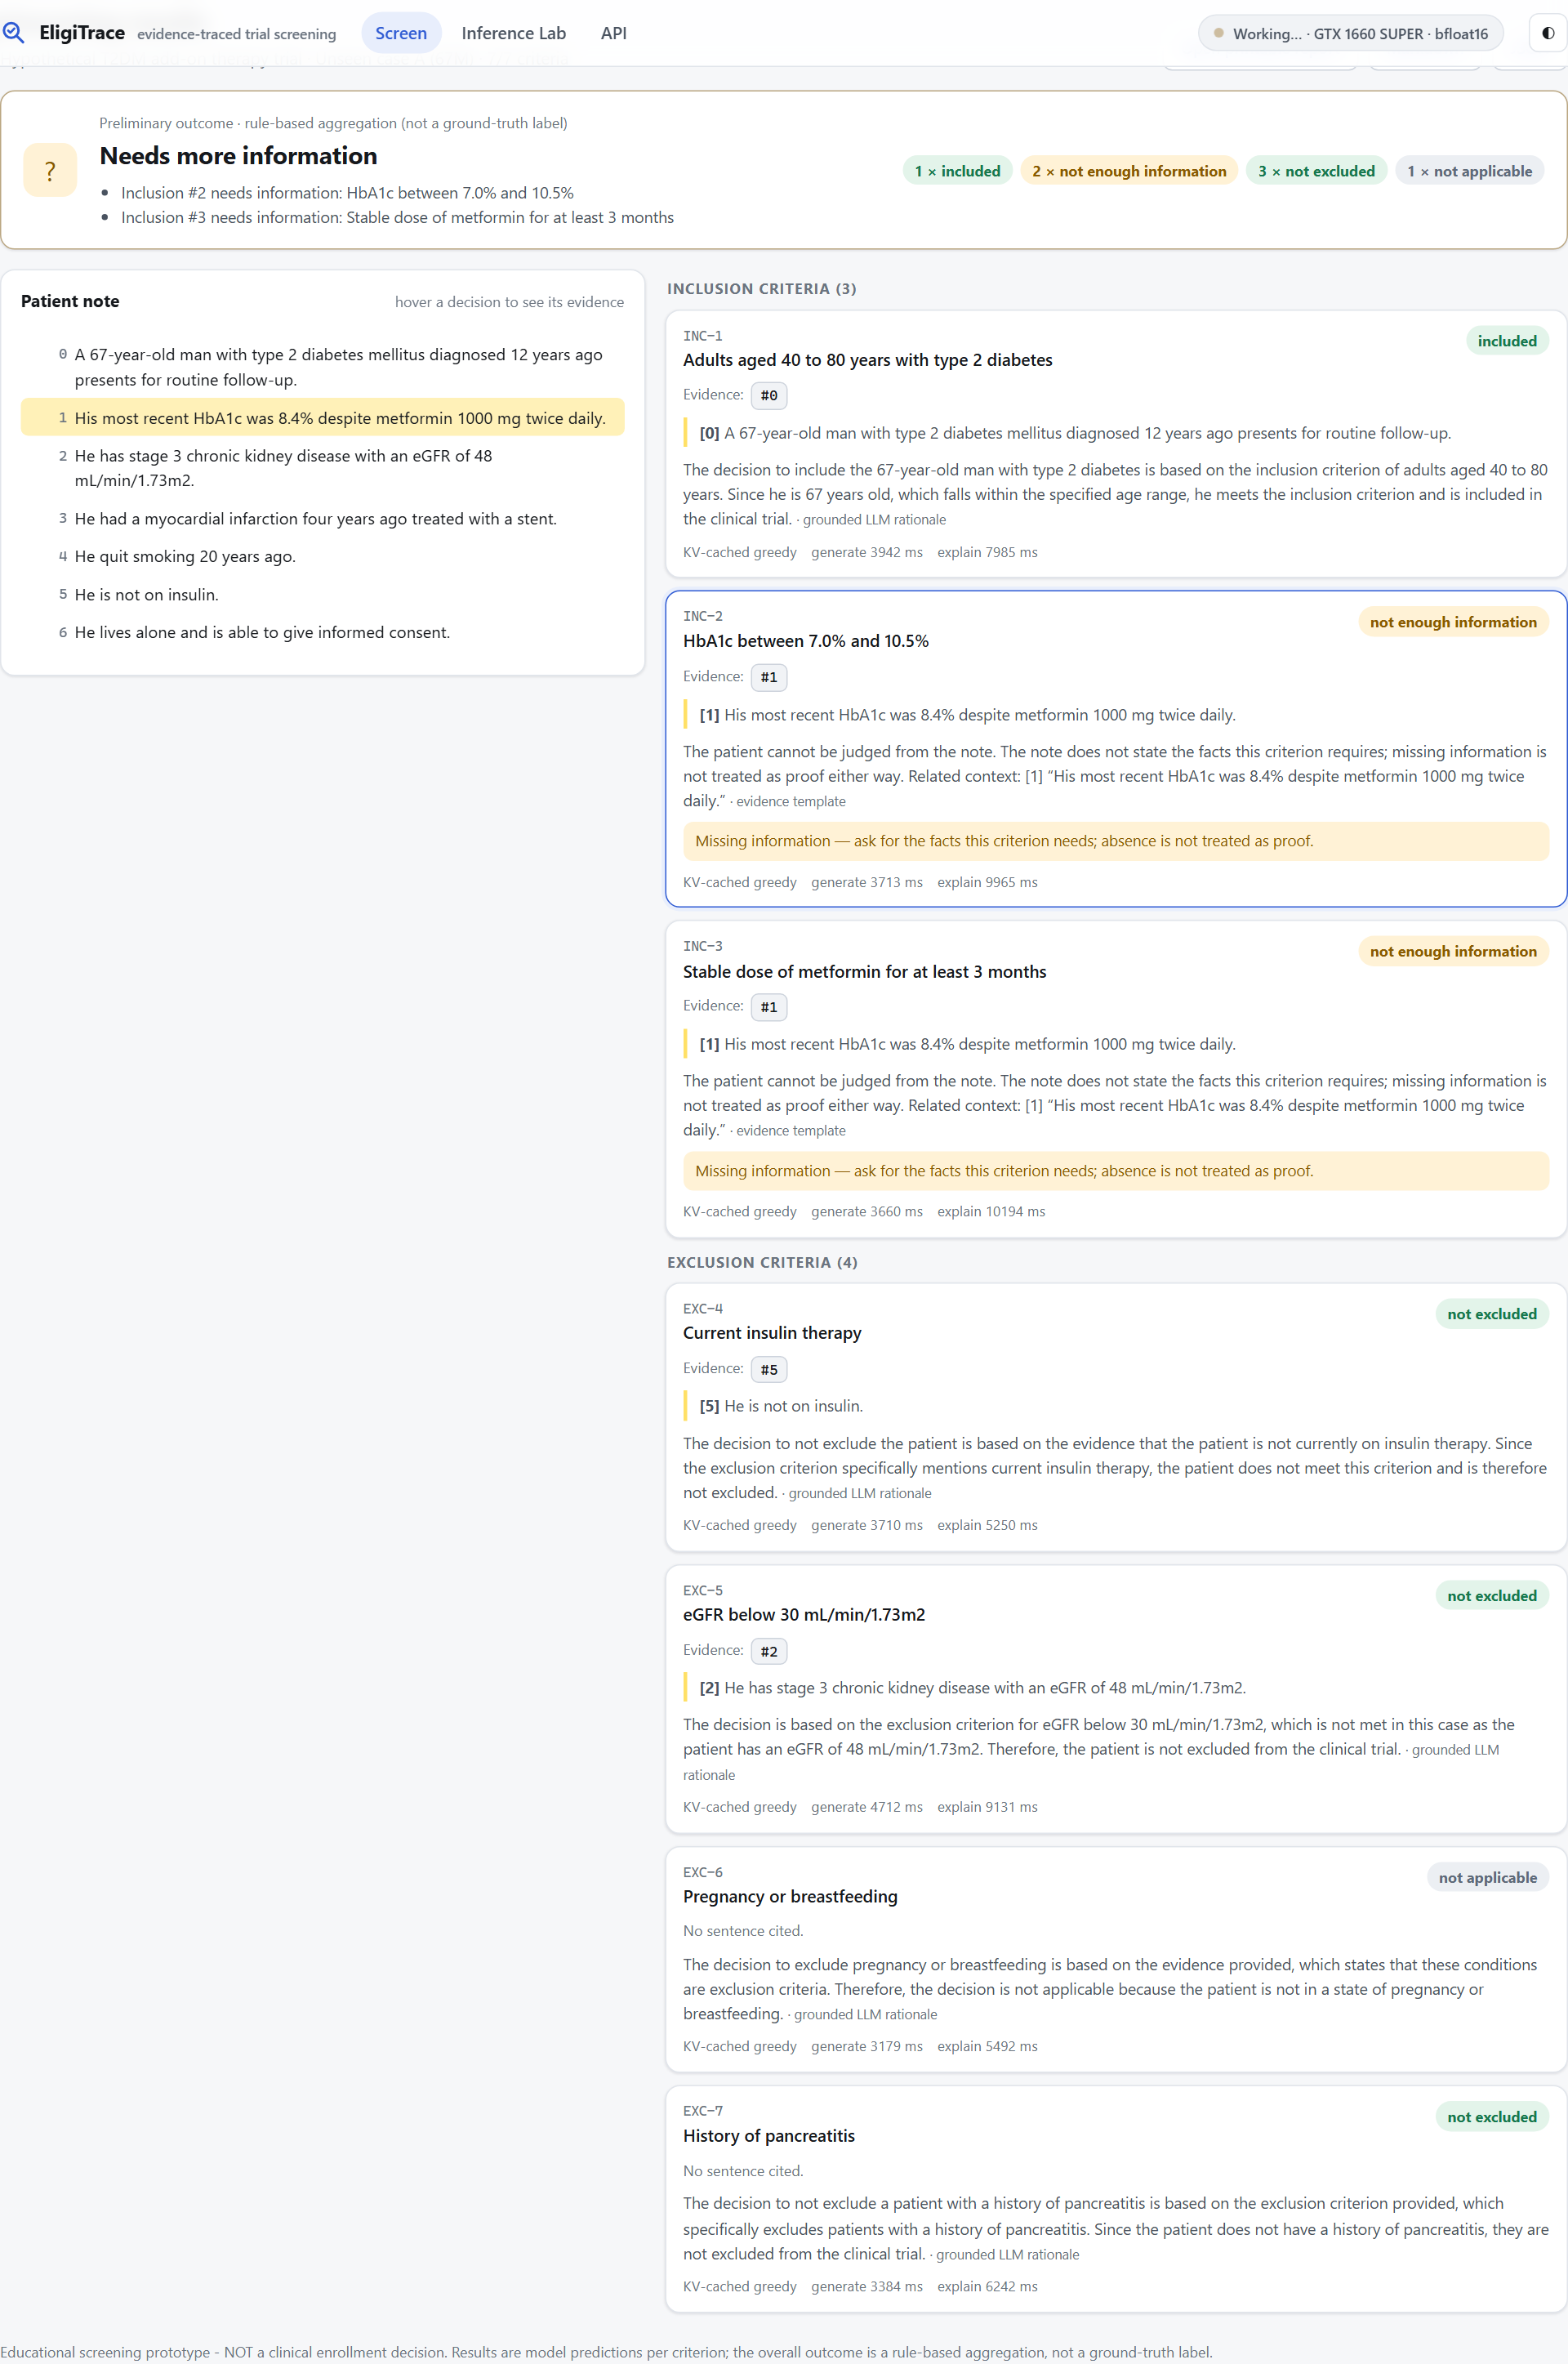
\includegraphics[width=0.49\linewidth]{screens/03_results.png}\\[4pt]
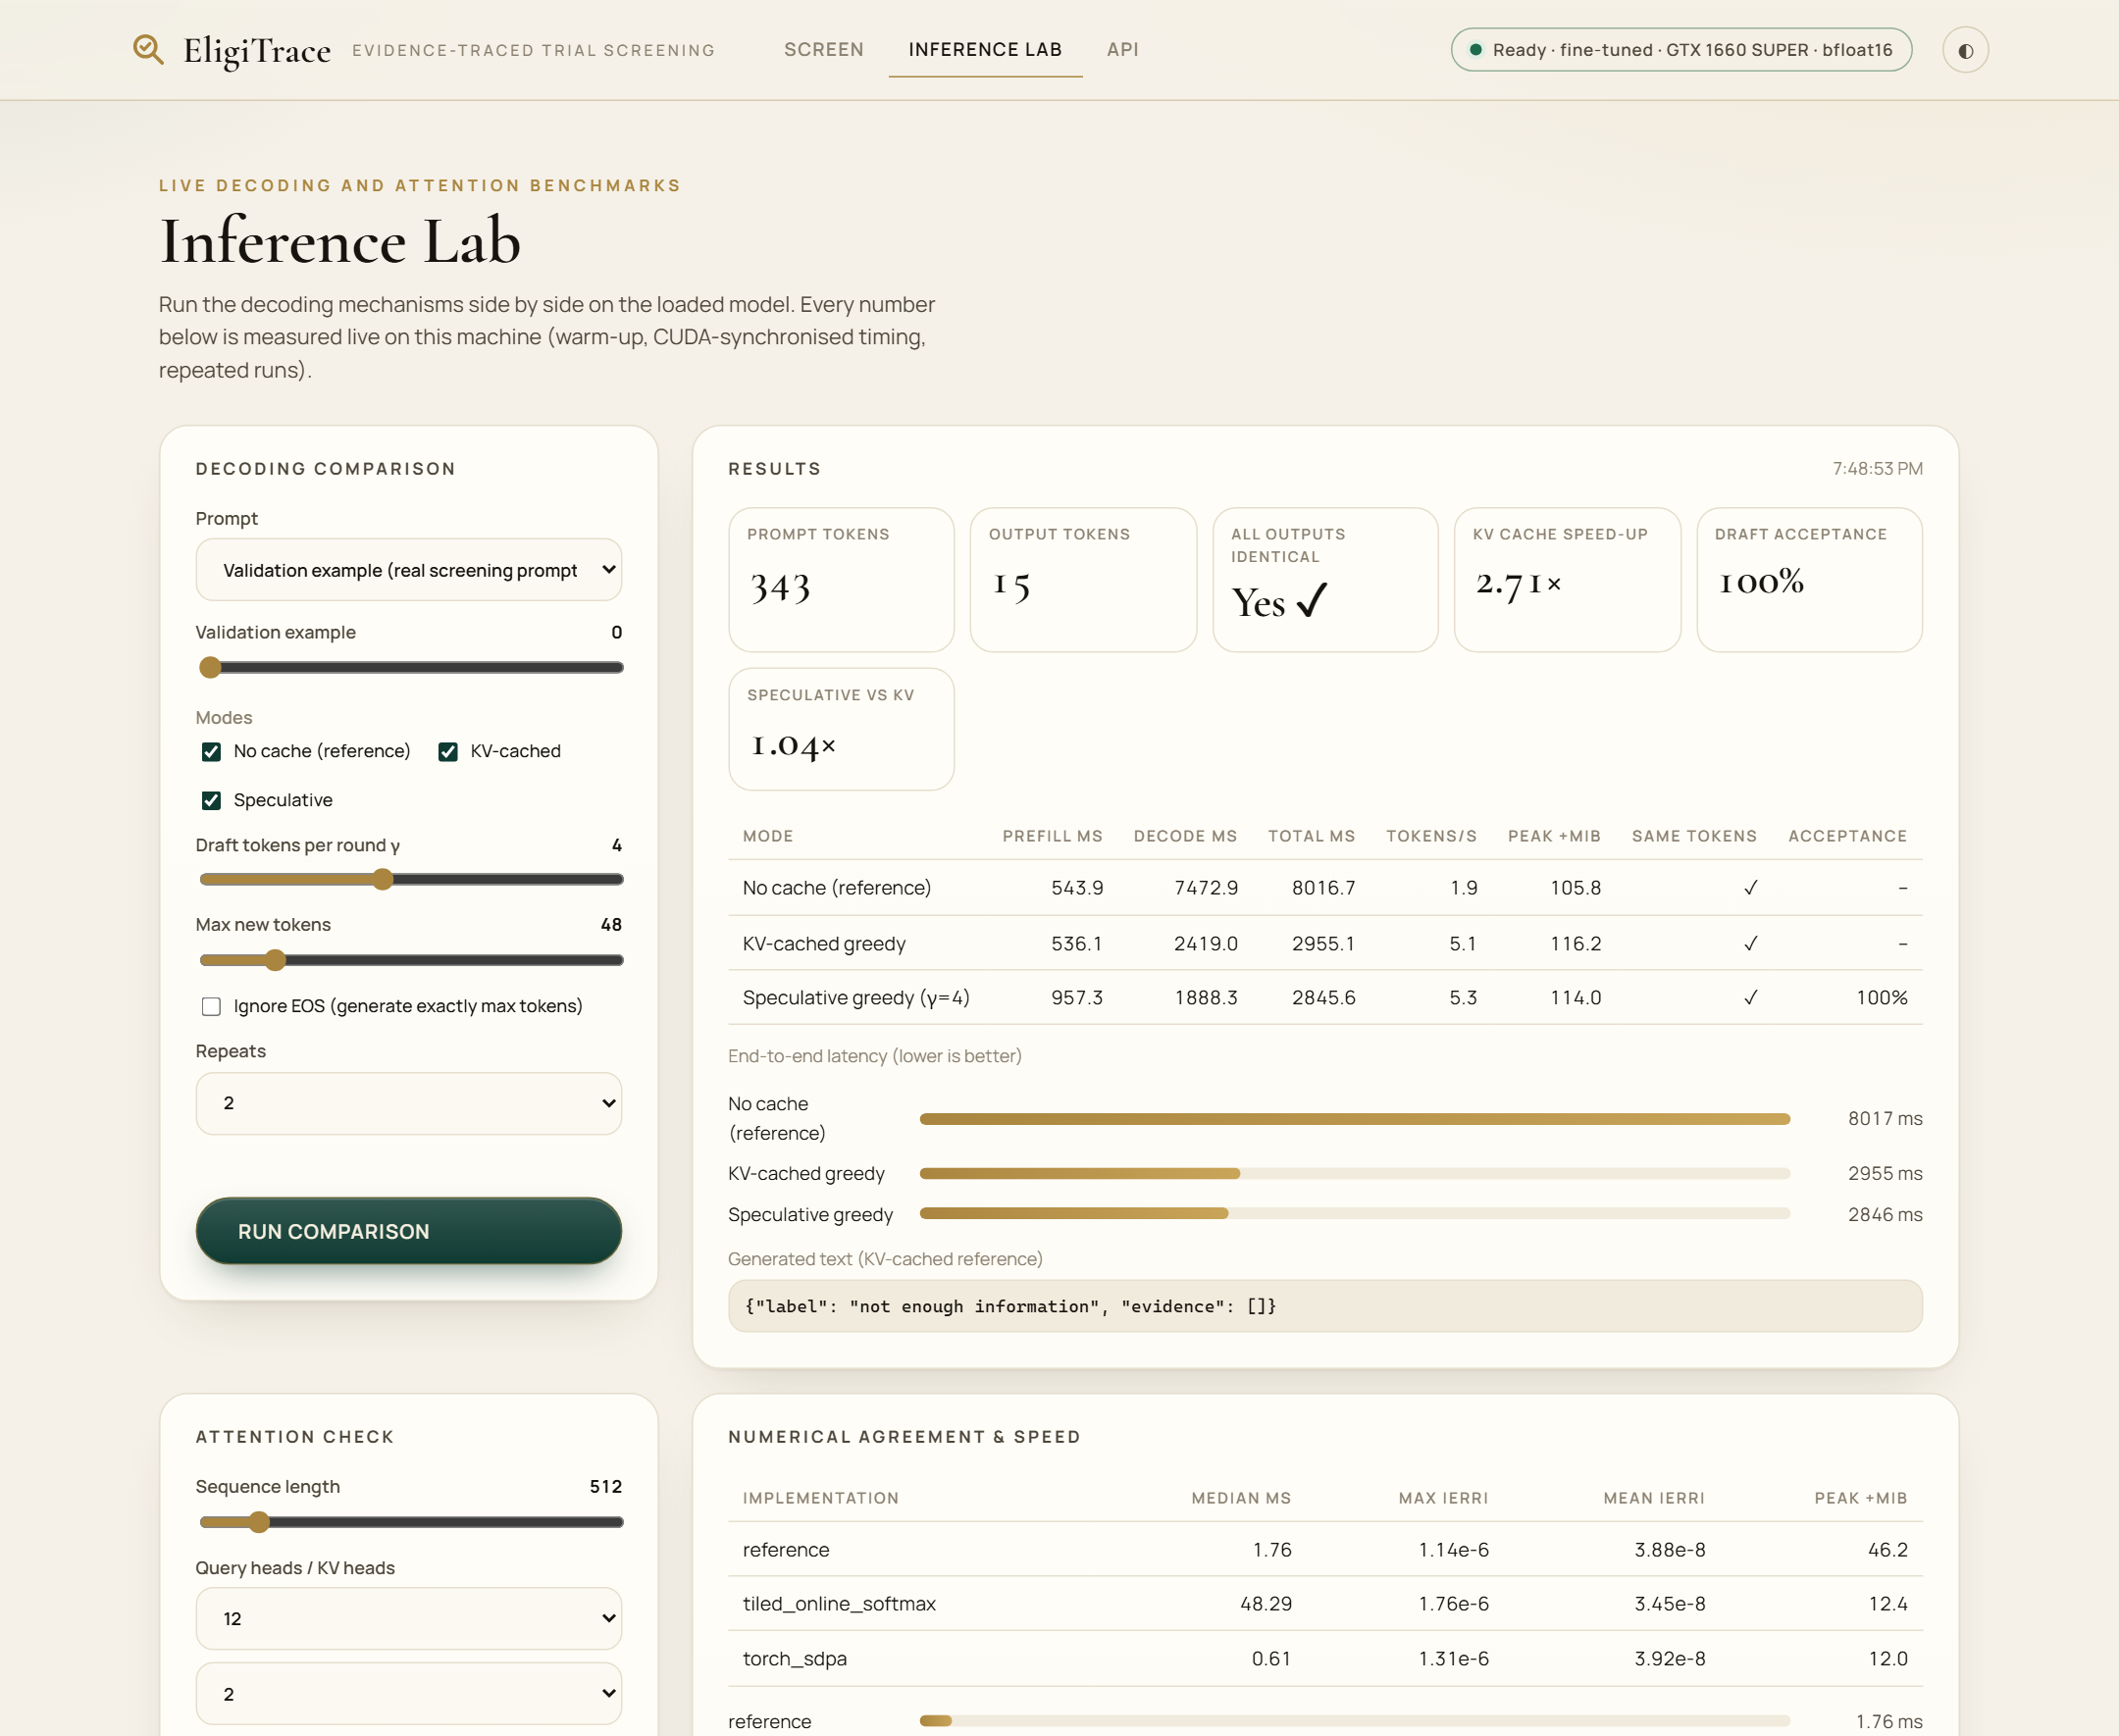
\includegraphics[width=0.49\linewidth]{screens/06_lab.png}\hfill
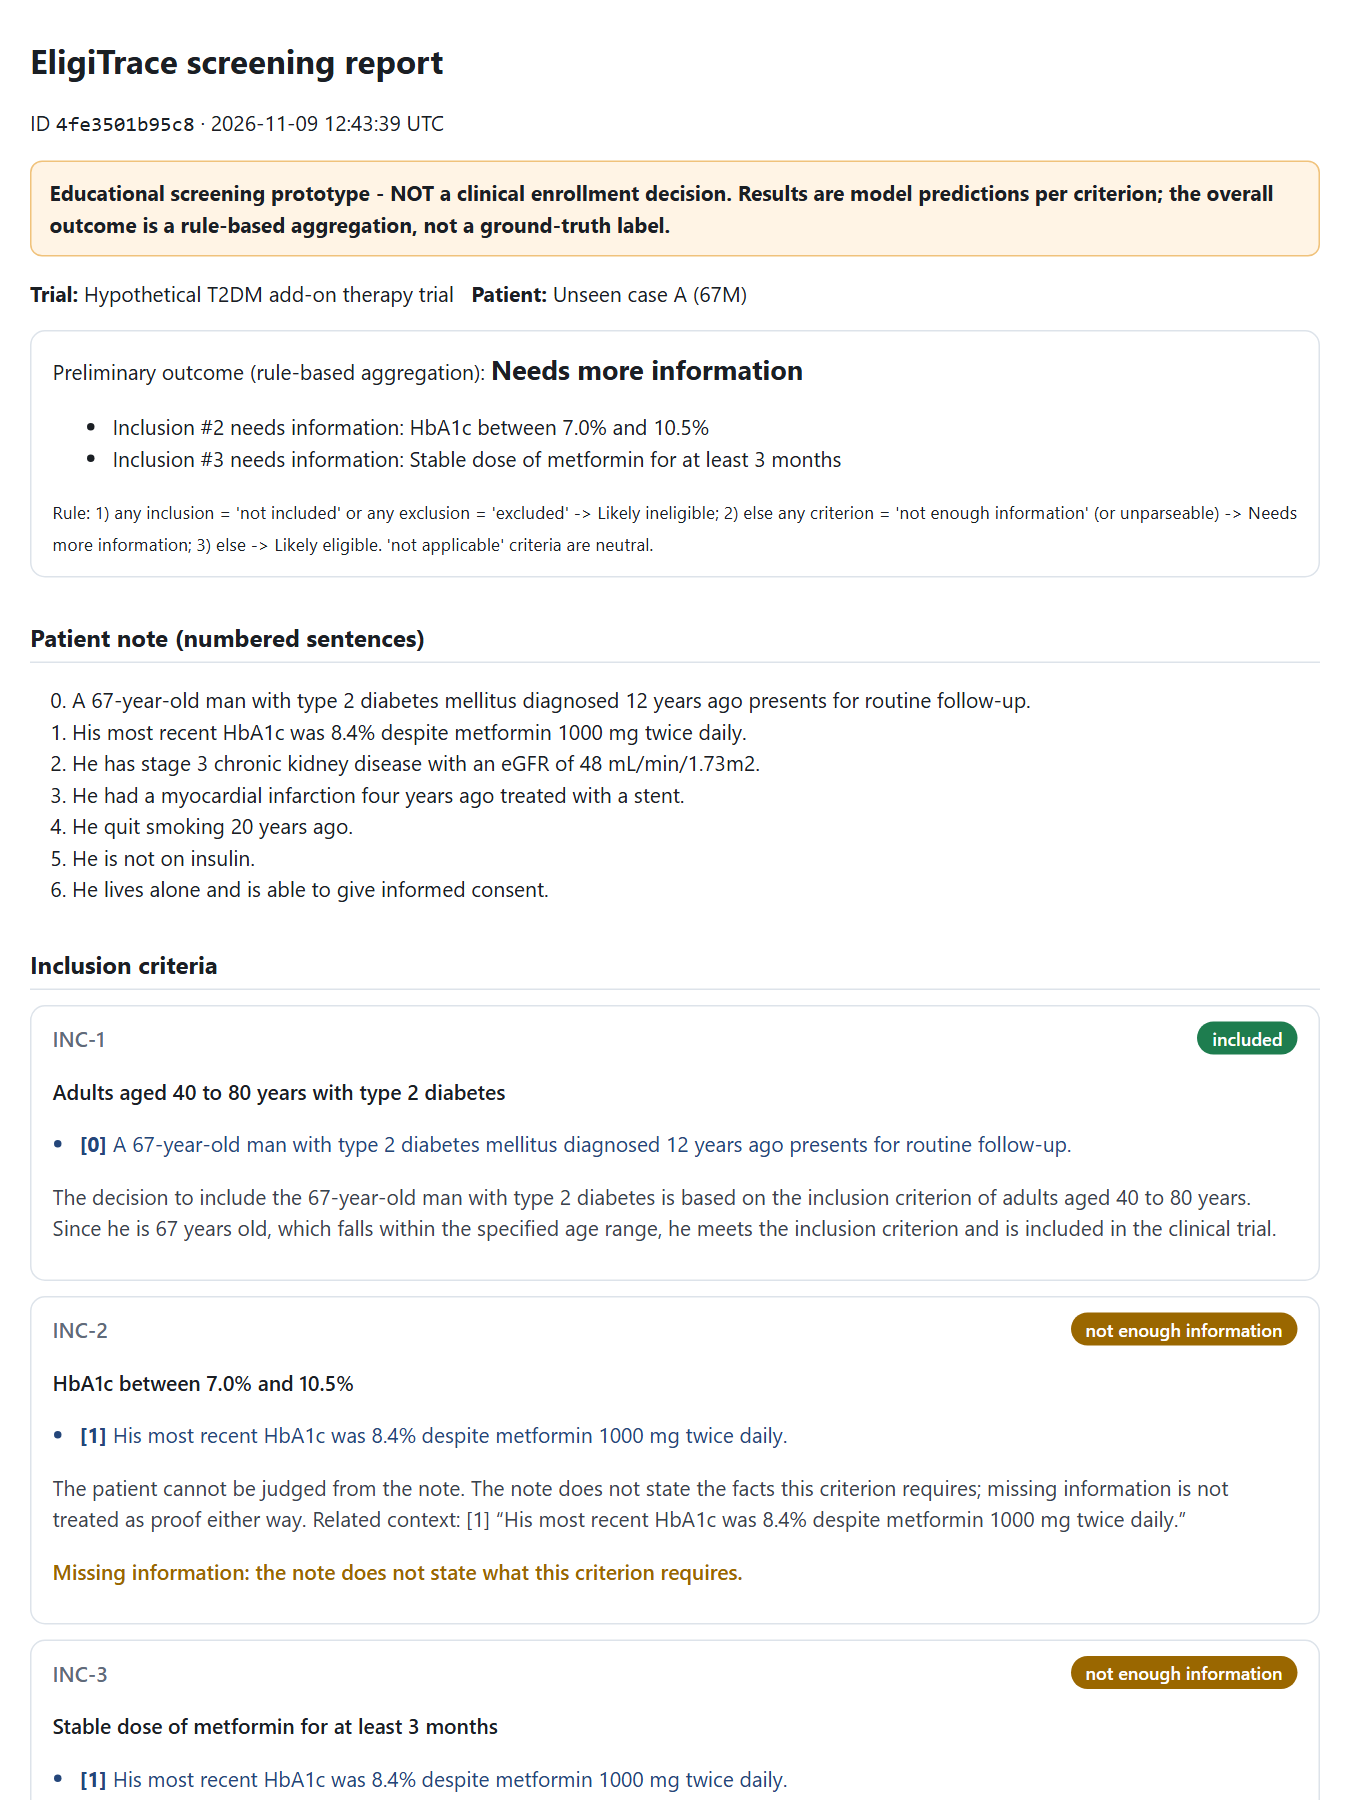
\includegraphics[width=0.49\linewidth]{screens/04_report.png}
\caption{\sys\ application. Top: input of an unseen note and criteria (left), and criterion results with
highlighted evidence, grounded rationales and the rule-based outcome (right). Bottom: Inference Lab with live
decoder and attention comparisons (left), and the exported report with provenance (right).}
\label{fig:app}
\end{figure*}


\section{Limitations}\label{sec:limits}
\textbf{Data scale and label skew.} The benchmark has 53 patients; the prescribed split leaves 603 training
annotations and only 8 test patients (206 annotations). Rare labels are nearly absent: the test split has no
\emph{excluded} example and only 7 \emph{not included}, so per-class scores for these classes are either
undefined or rest on a handful of cases, and patient-level bootstrap intervals are wide.

\textbf{Single seed, limited search.} Each training configuration was run once (seed 42) and the
hyper-parameter search was deliberately small to respect the 6\,GB budget and the deadline; reported
differences of a few points are within run-to-run variance we did not measure.

\textbf{Explanations.} Rationales are constrained to the cited sentences and pass an automatic grounding check,
but they were not rated by clinicians, and the check (numbers and label contradiction) cannot catch every
unfaithful paraphrase. They should be read as summaries of the cited evidence, not as clinical reasoning.

\textbf{Inference measurements.} Timings are from one consumer GPU under Windows with a slow host CPU; at
batch size 1 small kernels are launch-bound, which shapes every speed result (Section~\ref{sec:results}). The
tiled attention kernel is an educational PyTorch implementation, not a fused kernel, and was validated in
isolation rather than substituted into the production model path.

\textbf{Aggregation and scope.} The overall outcome is a hand-written rule over criterion predictions; the
dataset contains no patient--trial ground truth, so this outcome is not evaluated. Criteria fetched from
ClinicalTrials.gov are split heuristically. \sys\ is an educational screening prototype and must not be used
to make enrollment or treatment decisions.

\section{Conclusion}\label{sec:conclusion}
\sys\ shows that a 1.5B-parameter open model, adapted with LoRA on a single 6\,GB consumer GPU in about an
hour, reaches 0.733 accuracy on held-out patients and cites the same evidence sentences as expert annotators
far more precisely than its untuned starting point. Every component runs locally, so patient notes never leave
the machine.

Each inference mechanism has its own lesson:
\begin{itemize}
\item \emph{KV cache}: removes the quadratic cost of recomputation, and its benefit grows with context length;
\item \emph{online softmax}: removes the quadratic memory of attention, but needs kernel fusion before it also
saves time;
\item \emph{speculative decoding}: is exact, but at batch~1 on launch-bound hardware it only pays off when the
draft is much cheaper per step than the target, not merely smaller.
\end{itemize}
In reduced precision, agreement with the reference is ``identical up to ties within one rounding step'', and a
careful comparison has to say so explicitly.

The weakest areas are the rare labels and reasoning from the absence of a fact. Natural next steps are more
annotated data for \emph{not included} and \emph{not applicable}, label-balanced or contrastive training,
clinician review of the generated explanations, and a larger validation study: our three-seed runs show that
validation macro-F1 varies by about 0.16 between seeds, so single-run differences in the rare classes cannot be
trusted. Oversampling the rare labels, a fine-tuned draft model and a lower LoRA rank were all tested on the
validation split (Section~\ref{sec:res-extra}); none is shown to help beyond noise except that a fine-tuned
draft raises speculative acceptance from 0.59 to 0.85 (still slower than plain decoding).


\bibliographystyle{IEEEtran}
\bibliography{refs}

\appendices
\section{AI-Use Statement}\label{app:ai}
Claude (Anthropic) was used as an AI assistant to help with literature search, planning, code scaffolding,
debugging and drafting text. All code was reviewed, executed and tested by the author (the automated test
suite covers the data split, leakage, parser, metrics, attention, KV-cache and speculative-decoding equality,
and the API), all reported numbers come from runs in this repository, and the author can explain, execute and
modify every component. No AI-generated content was used as data, labels or evaluation signal.

\section{Reproducibility}\label{app:repro}
Source code, configuration, split manifest, logs and results: \url{https://github.com/ruhank-dev/eligitrace}.
LoRA adapter: \url{https://huggingface.co/arceus1rk/eligitrace-qwen2.5-1.5b-lora}.
With \texttt{uv} and \texttt{Task} installed:
{\footnotesize
\begin{verbatim}
task setup     # env from uv.lock
task data      # split, manifest, stats
task train     # LoRA fine-tuning
task eval-final  # one-time test eval
task bench-kv; task bench-attn
task bench-spec
task download-weights
task app       # 127.0.0.1:8000
\end{verbatim}
}


\end{document}
